\documentclass[a4paper,english]{lipics-v2016}
\usepackage{microtype}

%% This is our standard package for code formatting:
\usepackage{listings}
\usepackage{url}
\usepackage{amsmath}
\usepackage{amsthm}
\usepackage{hyperref}
\usepackage{graphicx}
% \usepackage{mathabx}
% \usepackage{mathpartir}
\usepackage{xspace}
\usepackage[noabbrev,capitalise]{cleveref}
\usepackage{enumitem}

\usepackage{wrapfig}

\usepackage[labelformat=simple]{subcaption}

%Re-formatting figure captions to make subfigures look right.
\newcommand{\myhrule}{ \leaders\hrule width 0pt height .33pt \hfill }
\renewcommand{\myhrule}{\hrulefill}

\DeclareCaptionFormat{ruled}{\myhrule \\ #1#2#3}
\DeclareCaptionFormat{plain}{#1#2#3}

\captionsetup[figure]{format=ruled}
\captionsetup[subfigure]{format=plain}

\newcommand{\treelang}{Gibbon\xspace} 
\newcommand{\treecomp}{Gibbon compiler{}}

%% Traversal effects:
\newcommand{\travarr}[1]{\xrightarrow{#1}}
% \newcommand{\arr}[3]{\ensuremath{{#1} \xrightarrow{\overrightarrow{#2}} {#3}}}
% \newcommand{\arr}[3]{\ensuremath{{#1} \xrightarrow{trav({#2})} {#3}}}
\newcommand{\arr}[3]{\ensuremath{{#1} \travarr{#2} {#3}}}
% $\xrightarrow[world]{hello}$



\renewcommand{\thesubfigure}{(\alph{subfigure})}

\newcommand{\fresh}[1]{\ensuremath{#1}}
\newcommand{\fixed}[1]{\ensuremath{\texttt{#1}}}

\newcommand{\freshA}{\fresh{\alpha}}
\newcommand{\freshB}{\fresh{\beta}}
\newcommand{\locend}[1]{\ensuremath{\hat{#1}}}

\newif\ifcurly
% \curlytrue % Comment to deactivate.

\newcommand{\finishmecurly}{\ifcurly \Red{FINISHME - do ifcurly version here} \else}


%----------------------------------------
%% \usepackage[colorinlistoftodos,prependcaption,textsize=tiny]{todonotes}
%% \usepackage{xargs}
%% \newcommandx{\unsure}[2][1=]{\todo[linecolor=red,backgroundcolor=red!25,bordercolor=red,#1]{#2}}
%% \newcommandx{\info}[2][1=]{\todo[linecolor=OliveGreen,backgroundcolor=OliveGreen!25,bordercolor=OliveGreen,#1]{#2}}
%% \newcommandx{\change}[2][1=]{\todo[linecolor=blue,backgroundcolor=blue!25,bordercolor=blue,#1]{#2}}
%% \newcommandx{\inconsistent}[2][1=]{\todo[linecolor=blue,backgroundcolor=blue!25,bordercolor=red,#1]{#2}}
%% \newcommandx{\improvement}[2][1=]{\todo[linecolor=Plum,backgroundcolor=Plum!25,bordercolor=Plum,#1]{#2}}
%% \newcommandx{\resolved}[2][1=]{\todo[linecolor=OliveGreen,backgroundcolor=OliveGreen!25,bordercolor=OliveGreen,#1]{#2}} % use this to mark a resolved question
%% \newcommandx{\thiswillnotshow}[2][1=]{\todo[disable,#1]{#2}} % will replace \resolved in the final document
% ----------------------------------------


% Tweak width of margin notes for this documentclass:
\setlength{\marginparwidth}{1.75cm}

% If we are using Haskell code in this paper:
% Defines ``code'' environment:
% 
\usepackage{upquote}
\usepackage{listings}
\usepackage[usenames,dvipsnames]{xcolor}

\definecolor{darkgreen}{rgb}{0,0.5,0}
\definecolor{darkred}{rgb}{0.5,0,0}

% Define the language styles we will use
%
\lstset{%
    frame=none,
    rulecolor={\color[gray]{0.7}},
    numbers=none,
    basicstyle=\ttfamily,        
%    basicstyle=\smallsize\ttfamily,    
%    basicstyle=\footnotesize\ttfamily,
%    basicstyle=\scriptsize\ttfamily,
%    basicstyle=\Largesize\ttfamily,        
    numberstyle=\color{Gray}\tiny\it,
    commentstyle=\color{MidnightBlue}\it,
    stringstyle=\color{Maroon},
    keywordstyle=[1],
    keywordstyle=[2]\color{ForestGreen},
    keywordstyle=[3]\color{Bittersweet},
    keywordstyle=[4]\color{RoyalPurple},
    captionpos=b,
    aboveskip=1\medskipamount,
    xleftmargin=0.5\parindent,
    xrightmargin=0.5\parindent,
    flexiblecolumns=false,
%   basewidth={0.5em,0.45em},           % default {0.6,0.45}
%    escapechar={\%},
    escapechar={\@},
    mathescape=true,
    texcl=true                          % tex comment lines
}

\lstloadlanguages{Haskell}
\lstdefinestyle{haskell}{%
    language=Haskell,
    upquote=true,
    basicstyle=\ttfamily,        
    deletekeywords={case,class,data,default,deriving,do,in,instance,let,of,type,where,IO,ST,STM,read},
%    morekeywords={[1]read,write,finish},
    morekeywords={[2]class,data,default,deriving,family,instance,type,where},
    morekeywords={[3]in,let,case,of,do,switch},
    morekeywords={[4]IORef,IO,ST,STM,Symbol},
    literate=
        {\\}{{$\lambda$}}1
        {\\\\}{{\char`\\\char`\\}}1
        {>->}{>->}3
        {>>=}{>>=}3
        {->}{{$\rightarrow$}}2
        {>=}{{$\geq$}}2
        {<-}{{$\leftarrow$}}2
        {<=}{{$\leq$}}2
        {=>}{{$\Rightarrow$}}2
        {|}{{$\mid$}}1
        {forall}{{$\forall$}}1
        {exists}{{$\exists$}}1
        {...}{{$\cdots$}}3
%       {`}{{\`{}}}1
%       {\ .}{{$\circ$}}2
%       {\ .\ }{{$\circ$}}2
%
%    deletekeywords={insert},
%    deletekeywords={map,sort,zipWith,replicate,Num,Char,Bool,Array,Int,Double
%                   ,sqrt,not,filter,IO,Maybe,Either,quot,scanl,scanr,reverse,fst,id},
%    literate=
%        {+}{{$+$}}1
%        {/}{{$/$}}1
%        {*}{{$*$}}1
%        % {=}{{$=$}}1
%        {>}{{$>$}}1 {<}{{$<$}}1
%        {\\}{{$\lambda$}}1
%        {\\\\}{{\char`\\\char`\\}}1
%        {->}{{$\rightarrow\;$}}2
%        {>=}{{$\geq$}}2
%        {<-}{{$\leftarrow\;$}}2
%        {<=}{{$\leq$}}2
%        {=>}{{$\Rightarrow\;$}}2
%        {\ .}{{$\circ$}}2
%        {\ .\ }{{$\circ$}}2
%        {>>}{{>>}}2
%        {>>=}{{>>=}}2
%        {=<<}{{=<<}}2
%        {|}{{$\mid$}}1
%        {dotdotdot}{{$\ldots$}}3
}

\lstdefinestyle{inline}{%
    style=haskell,
%    basicstyle=\footnotesize\ttfamily,
    basicstyle=\ttfamily,
    %% keywordstyle=[1],
    %% keywordstyle=[2],
    %% keywordstyle=[3],
    %% keywordstyle=[4],
    literate=
        {\\}{{$\lambda$}}1
        {\\\\}{{\char`\\\char`\\}}1
        {>->}{>->}3
        {>>=}{>>=}3
        {->}{{$\rightarrow$\space}}3    % include forced space
        {>=}{{$\geq$}}2
        {<-}{{$\leftarrow$}}2
        {<=}{{$\leq$}}2
        {=>}{{$\Rightarrow$}}2
        {|}{{$\mid$}}1
%        {~}{{$\sim$}}1
        {forall}{{$\forall$}}1
        {exists}{{$\exists$}}1
        {...}{{$\cdots$}}3
}

\lstnewenvironment{code}
    {\lstset{style=haskell}%
      \csname lst@SetFirstLabel\endcsname}
    {\csname lst@SaveFirstLabel\endcsname}
    {}

% Default all listings to Haskell style
\lstset{style=haskell}

% \newcommand{\inl}[1]{\lstinline[style=inline];#1;}
\newcommand{\il}[1]{\lstinline[style=inline];#1;}

\newcommand{\makeatcode}{\lstMakeShortInline[style=inline]@}
\newcommand{\makeatchar}{\lstDeleteShortInline@}


\usepackage{upquote}
\usepackage{listings}
\usepackage[usenames,dvipsnames]{xcolor}

\definecolor{darkgreen}{rgb}{0,0.5,0}
\definecolor{darkred}{rgb}{0.5,0,0}

% Define the language styles we will use
%
\lstset{%
    frame=none,
    rulecolor={\color[gray]{0.7}},
    numbers=none,
    basicstyle=\ttfamily,        
%    basicstyle=\smallsize\ttfamily,    
%    basicstyle=\footnotesize\ttfamily,
%    basicstyle=\scriptsize\ttfamily,
%    basicstyle=\Largesize\ttfamily,        
    numberstyle=\color{Gray}\tiny\it,
    commentstyle=\color{MidnightBlue}\it,
    stringstyle=\color{Maroon},
    keywordstyle=[1],
    keywordstyle=[2]\color{ForestGreen},
    keywordstyle=[3]\color{Bittersweet},
    keywordstyle=[4]\color{RoyalPurple},
    captionpos=b,
    aboveskip=1\medskipamount,
    xleftmargin=0.5\parindent,
    xrightmargin=0.5\parindent,
    flexiblecolumns=false,
%   basewidth={0.5em,0.45em},           % default {0.6,0.45}
%    escapechar={\%},
    escapechar={\@},
    mathescape=true,
    texcl=true                          % tex comment lines
}

\lstloadlanguages{Haskell}
\lstdefinestyle{haskell}{%
    language=Haskell,
    upquote=true,
    basicstyle=\ttfamily,        
    deletekeywords={case,class,data,default,deriving,do,in,instance,let,of,type,where,IO,ST,STM,read},
%    morekeywords={[1]read,write,finish},
    morekeywords={[2]class,data,default,deriving,family,instance,type,where},
    morekeywords={[3]in,let,case,of,do,switch},
    morekeywords={[4]IORef,IO,ST,STM,Symbol},
    literate=
        {\\}{{$\lambda$}}1
        {\\\\}{{\char`\\\char`\\}}1
        {>->}{>->}3
        {>>=}{>>=}3
        {->}{{$\rightarrow$}}2
        {>=}{{$\geq$}}2
        {<-}{{$\leftarrow$}}2
        {<=}{{$\leq$}}2
        {=>}{{$\Rightarrow$}}2
        {|}{{$\mid$}}1
        {forall}{{$\forall$}}1
        {exists}{{$\exists$}}1
        {...}{{$\cdots$}}3
%       {`}{{\`{}}}1
%       {\ .}{{$\circ$}}2
%       {\ .\ }{{$\circ$}}2
%
%    deletekeywords={insert},
%    deletekeywords={map,sort,zipWith,replicate,Num,Char,Bool,Array,Int,Double
%                   ,sqrt,not,filter,IO,Maybe,Either,quot,scanl,scanr,reverse,fst,id},
%    literate=
%        {+}{{$+$}}1
%        {/}{{$/$}}1
%        {*}{{$*$}}1
%        % {=}{{$=$}}1
%        {>}{{$>$}}1 {<}{{$<$}}1
%        {\\}{{$\lambda$}}1
%        {\\\\}{{\char`\\\char`\\}}1
%        {->}{{$\rightarrow\;$}}2
%        {>=}{{$\geq$}}2
%        {<-}{{$\leftarrow\;$}}2
%        {<=}{{$\leq$}}2
%        {=>}{{$\Rightarrow\;$}}2
%        {\ .}{{$\circ$}}2
%        {\ .\ }{{$\circ$}}2
%        {>>}{{>>}}2
%        {>>=}{{>>=}}2
%        {=<<}{{=<<}}2
%        {|}{{$\mid$}}1
%        {dotdotdot}{{$\ldots$}}3
}

\lstdefinestyle{inline}{%
    style=haskell,
%    basicstyle=\footnotesize\ttfamily,
    basicstyle=\ttfamily,
    %% keywordstyle=[1],
    %% keywordstyle=[2],
    %% keywordstyle=[3],
    %% keywordstyle=[4],
    literate=
        {\\}{{$\lambda$}}1
        {\\\\}{{\char`\\\char`\\}}1
        {>->}{>->}3
        {>>=}{>>=}3
        {->}{{$\rightarrow$\space}}3    % include forced space
        {>=}{{$\geq$}}2
        {<-}{{$\leftarrow$}}2
        {<=}{{$\leq$}}2
        {=>}{{$\Rightarrow$}}2
        {|}{{$\mid$}}1
%        {~}{{$\sim$}}1
        {forall}{{$\forall$}}1
        {exists}{{$\exists$}}1
        {...}{{$\cdots$}}3
}

\lstnewenvironment{code}
    {\lstset{style=haskell}%
      \csname lst@SetFirstLabel\endcsname}
    {\csname lst@SaveFirstLabel\endcsname}
    {}

% Default all listings to Haskell style
\lstset{style=haskell}

% \newcommand{\inl}[1]{\lstinline[style=inline];#1;}
\newcommand{\il}[1]{\lstinline[style=inline];#1;}

\newcommand{\makeatcode}{\lstMakeShortInline[style=inline]@}
\newcommand{\makeatchar}{\lstDeleteShortInline@}
 

% Copy this if needed to customize:
\input{./bibs/latex_templates/editingmarks}

\lstloadlanguages{C++}
\lstnewenvironment{cpp}
    {\lstset{}%
      \csname lst@SetFirstLabel\endcsname}
    {\csname lst@SaveFirstLabel\endcsname}
    \lstset{
      language=C++,
%      basicstyle=\footnotesize\ttfamily,
      basicstyle=\ttfamily,              
%      basicstyle=\small\ttfamily,
      flexiblecolumns=false,
      basewidth={0.5em,0.45em},
      keywordstyle=\color{blue},
      % commentstyle=\color{darkgreen},
      commentstyle=\color{MidnightBlue}\it,
      morekeywords={uint64_t, ticks, ticks_t, avg_t, histogram_t, stack_t, sync,
      long_spawn, fun, match}
      % deletekeywords={map,sort,zipWith,replicate,Num,Char,Bool,Array,Int,Double
      %                ,sqrt,not,filter,IO,Maybe,Either,quot,scanl,scanr,reverse,fst,id},
      % literate= {+}{{$+$}}1 {/}{{$/$}}1 {*}{{$*$}}1 % {=}{{$=$}}1
      %           {>}{{$>$}}1 {<}{{$<$}}1
      %          {\\}{{$\lambda$}}1
      %          {\\\\}{{\char`\\\char`\\}}1
      %          {->}{{$\rightarrow$}}2 {>=}{{$\geq$}}2 {<-}{{$\leftarrow$}}2
      %          {<=}{{$\leq$}}2 {=>}{{$\Rightarrow$}}2
      %          {\ .}{{$\circ$}}2 {\ .\ }{{$\circ$}}2
      %          {>>}{{>>}}2 {>>=}{{>>=}}2 {=<<}{{=<<}}2
      %          {|}{{$\mid$}}1
      %          {dotdotdot}{{$\ldots$}}3
    }
    
% Sometimes we have extra short-cuts:
% \input{macro-defs}

% Sometimes we factor large figures into commands in a separate file:
% \input{figures}



%\special{papersize=8.5in,11in}
%\setlength{\pdfpageheight}{\paperheight}
%\setlength{\pdfpagewidth}{\paperwidth}

%\conferenceinfo{CONF 'yy}{Month d--d, 20yy, City, ST, Country}
%\copyrightyear{20yy}
%\copyrightdata{978-1-nnnn-nnnn-n/yy/mm}
%\copyrightdoi{nnnnnnn.nnnnnnn}

% Uncomment the publication rights you want to use.
%\publicationrights{transferred}
%\publicationrights{licensed}     % this is the default
%\publicationrights{author-pays}

%\titlebanner{banner above paper title}        % These are ignored unless
%\preprintfooter{short description of paper}   % 'preprint' option specified.

\title{Compiling tree transforms to operate on packed representations}
% \subtitle{Faster compiler passes, parallelization ready}

%\authorinfo{Name1}
%           {Affiliation1}
%           {Email1}
%\authorinfo{Name2\and Name3}
%           {Affiliation2/3}
%           {Email2/3}

\author[1]{}
\Copyright{}%mandatory, please use full first names. LIPIcs license is "CC-BY";  http://creativecommons.org/licenses/by/3.0/
%

\lstMakeShortInline[style=inline]@
% \lstDeleteShortInline@

\begin{document}

\maketitle

\begin{abstract}
When written idiomatically in most programming languages, programs that traverse
and construct trees operate over pointer-based data structures, using one heap
object per-leaf and per-node.
%
{This representation is efficient for random access and shape-changing
  modifications, but for traversals, such as compiler passes, that process most
  or all of a tree in bulk, it can be inefficient.
%
In this work we instead compile tree traversals}
to operate on \textbf{pointer-free
pre-order serializations of trees}.  On modern architectures such programs
often run {significantly} faster than their pointer-based counterparts,
{and additionally are directly suited to storage and transmission without
  requiring marshaling.}

We present a prototype compiler, \textsf{Gibbon}, that compiles a small
first-order, purely functional language sufficient for tree traversals.
The compiler transforms this language into intermediate representation with
explicit pointers into input and output buffers
for packed data.
% , which then generates code as efficient as hand-written C.
%
The key compiler technologies include an effect
system for capturing traversal behavior, combined with an
algorithm to insert destination cursors.
% lightweight
% {analysis inferring data flow},
% and a program synthesis step for
% creating missing traversals.
We evaluate our compiler on 
tree transformations over a real-world dataset of source-code syntax trees.
%
{For traversals touching the whole tree, such as maps and folds, packed data
  allows speedups of over $2\times$ compared to a highly-optimized pointer-based
  baseline.}

\end{abstract}

%\category{CR-number}{subcategory}{third-level}

% general terms are not compulsory anymore,
% you may leave them out
%\terms
%term1, term2

%\keywords
%keyword1, keyword2

% ================================================================================
\section{Introduction}\label{sec:intro}
% ================================================================================

% \rn{This is an example peanut-gallery comment.}

Programs that traverse and construct trees are widely used across all
domains of computer science, ranging from compiler passes, to the
browser Document Object Model, to particle simulations with
space-partitioning trees.
%
Yet almost all modern programming languages and
compilers represent trees and their traversals identically.
% In the traditional representation,
Each node of the tree is a heap object, followed by fields for child nodes or
leaf values.  This representation has not changed since early LISP systems and
is shared across source languages with diverse type
systems---whether algebraic data types or class hierarchies, statically or
dynamically typed.  The deviations from this consensus are found within
limited high-performance scenarios where complete trees can be laid out using
address arithmetic with no intermediate nodes.

We submit that this consensus is premature.  In numerical computing it is an axiom
that you cannot treat the numbers in a matrix as individual heap objects.
Rather, the emphasis is on bulk efficiency.  Likewise, many tree traversals
process trees in bulk, reading or writing them in one pass.  On such workloads,
traditional tree representations are not favored by current trends in computer
architecture.  Pointer-chasing implies randomized memory access patterns.
%
While previous work addresses spatial locality for tree data~\cite{Chilimbi1999},
%
much memory is still wasted both in pointers themselves and in tags on nodes
(e.g. distinguishing ``interior'' vs ``leaf'' objects).  For example, a C
compiler uses 96 bytes
%
%% \rn{Double check that for alignment the C compiler is sacrificing a word for the
%% one byte tag field.} 
%
of memory to represent the tree shown in
Figure~\ref{fig:intro-tree-unpacked}. On the other hand, if we are
sending the tree over the network, we would naturally use a more
compact form in serializing it, as shown in
Figure~\ref{fig:intro-tree-packed}.  In the latter version, we use the
same 24 bytes for the data in the leaves, but only 5 bytes for the
spine (capturing the ``tags'' of the 5 nodes in the tree), rather than
72.  Further, a tree traversal processing this memory representation
follows a precisely linear memory access pattern, because the data is
already laid out in a preorder traversal.
%
On architectures with inexpensive unaligned access, such as modern
x86, this is a desirable in-memory representation as well as a
serialization format.\footnote{Even restricted to aligned access, we
  would still shrink from 72 bytes to 20 by switching to a packed
  format.}

\begin{figure}
  \begin{subfigure}[t]{\linewidth}
    \centering
    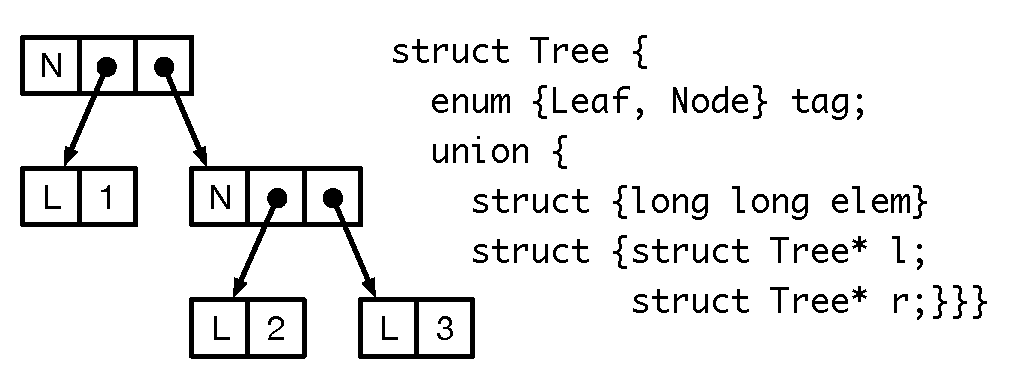
\includegraphics[scale=0.5]{figs/intro-tree-unpacked}
    \caption{Standard representation of a tree structure in C}
    \label{fig:intro-tree-unpacked}
  \end{subfigure}
  \begin{subfigure}[t]{\linewidth}
    \centering
    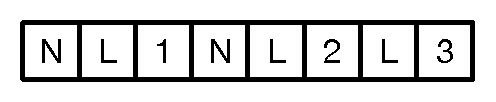
\includegraphics[scale=0.5]{figs/intro-tree-packed}
    \caption{Serialized version of the same tree}
    \label{fig:intro-tree-packed}    
  \end{subfigure}
  \caption{Standard and serialized representations of trees}
  \label{fig:intro-fig}
\end{figure}

% \begin{figure}
%% \begin{figure}
%% %\begin{wrapfigure}{r}{0.5\textwidth} 
%% {PICTURE HERE:  possibly with wrapfig.}
% \begin{verbatim}
%  [N|.|.]          struct Tree {
%     /  \           enum { Leaf, Node } tag;
% [L 1]  [N|.|.]     union { 
%          /   \      struct { long long elem; };
%       [L 2] [L 3]   struct { struct Tree* l;
%                              struct Tree* r; }}}
% \end{verbatim}

%%   \caption{Traditional, pointer-based tree layout.}
%% \end{figure}
%\end{wrapfigure}
% \begin{verbatim}
%   [N L 1  N L 2  L 3 ]
% \end{verbatim}
% \end{figure}

Indeed, if we can compile programs to operate directly on this serialization, we
follow a precedent of using serialization formats jointly as memory formats.
For example, Cap'N Proto \cite{capnproto} makes it ergonomic for C++ code to operate directly
on the Protobuf serialization format in memory.  Likewise ``data baking''\footnote{Described here \url{http://nullprogram.com/blog/2016/11/15/}}.
 is an established practice in video games---caching assets on
disk in a format that allows them to be \il{mmap}'d into memory and used
without further conversion.  As a general example of this capability, the
Glasgow Haskell Compiler (GHC) recently added the capability to store any closed
subgraph of the heap as a {\em Compact Normal Form} (CNF) \cite{cnf-icfp15}---a
contiguous memory region that is treated as a kind of ``super heap object'', never
traced by the GC and collected only when there are no pointers into any of the
sub-parts of the CNF.

The packed tree format above is precisely a dense encoding of a CNF---a
transitive closure of heap objects with no escaping pointers, in this case, no
pointers {\em at all}.  GHC's CNF support---like related efforts at
region~\cite{mlkit} or pool memory management~\cite{Lattner2005}---colocates
heap objects without changing their representation.
%
Code accessing the data can remain unchanged.
In contrast, the dense tree format {\em requires a complete
rearrangement of the compiled code that operates on the data}. This
rearrangement is fundamental to the space savings and format
simplicity.
% ---in contrast, CNF retains all of the pointers and tags of the original data.

% Shall we acronymize it?
% DTF - dense tree form, or dense tree format
% PTF - packed tree form
% DTP - dense tree packing

In this paper, we take a first step towards compiler support for 
packed tree data types {\em without} changing the source program.
%
Packed representations aren't always appropriate, and we don't automate the
choice of {\em when} to use them, but rather automate the necessary code
transformations to transparently use packed representations for selected
data types.
%
Henceforth, we use {\em tree traversals} or {\em tree transforms} to refer to
programs that walk over an immutable tree, building an output tree of size
proportional to the input tree, without substantially relying on {\em sharing}
in the representation.  We also address a limited class of {\em tree
  searches} that require random access within a tree.
%
We make the following contributions:

\newcommand{\calculus}{$\lambda^D_T$} % uh, Dense Tree?

\begin{itemize}
 %% \item We use a small core language, \calculus{}, to formalize a transformation
  %% on programs that creates an output program operating only on
  %% pointers in the serialized representation.  This involves a small program
  %% synthesis step, and we show how the program synthesis and the selection of
  %% data structure shape benefit from co-optimization.
   
\item We present a compiler, dubbed \treelang, 
  that can compile a range of tree transforms, written in a minimal functional language,
 to be {more than twice as} fast as standard techniques (Section~\ref{sec:language}).
 We evaluate \treelang against both a number of existing compilers and
 its own best performance (without packing) in \cref{sec:eval}.

\item We present compilation algorithms for data packing (\cref{sec:compiler}),
  including a method for determining when a function reaches the end of its
  input(s), and for converting to a destination-cursor-passing style, which
  supports operating on data in dense byte streams.

%% \item We show that the principle of packed-tree traversals works
%%   broadly across a variety of language implementations, by benchmarking simple
%%   handwritten packed-tree programs~\cref{sec:eval-shootout} and
%%   demonstrating speedup even \emph{without} compiler support.
%% \rn{This implies we will show results for GHC/Packed, which we don't currently.}
  
\item In an additional evaluation, we show that not only can tree traversals
  become faster in the packed representation, but that they are still amenable
  to parallel speedup (\cref{sec:eval-parallel}).  To leverage parallelism, we
  need random access and thus extra layout information in dense encodings---a
  feature that also allows tree searches to be expressed in our framework, such
  as a point correlation application evaluated in \cref{sec:eval-kdtree}.
% \rn{Need to include the KDTree business in the speculative part}
  
\end{itemize}


% ================================================================================
% \section{Motivating Example}
\section{Background and Example}\label{sec:background}
% ================================================================================

We begin our study of packed tree representations with perhaps the
simplest example: binary trees with
integer leaves.
%
In a language with algebraic data types,
% In a strongly typed functional language,
a recursive walk on
the tree would typically use pattern matching, which we
demonstrate with the following function that increments each
integer leaf by one. 

\ifcurly
% [language=python]
\begin{code}[language=c]
type Tree = Leaf(Int) | Node(Tree,Tree);

fun add1(t) {
  match(t) {
    Leaf(n):   return Leaf(n+1);
    Node(x,y): return Node(add1(x),add1(y));
  }}
\end{code}
\else
\begin{code}
 data Tree = Leaf Int | Node Tree Tree
  
 add1 t = case t of
            Leaf n   -> Leaf (n+1)
            Node x y -> Node (add1 x) (add1 y)
\end{code}
\fi

\ifcurly
In fact,
\else
Here we use a Haskell-like syntax, but in fact
\fi
 the small, strict, first-order, purely functional language of tree traversals
we consider in this paper is already a subset of most existing languages.
The above program is not substantially different in C, Haskell, ML, F\#, Scala,
Swift, Rust, etc.  Only the details of switching on sum types (tagged unions)
differ, as well as the syntax for constructing an object while initializing its
fields, here: 
\ifcurly
\il{Node(e1,e2)}).
\else
\il{Node e1 e2}.
\fi

%% For the purposes of establishing the problems we solve, and for explaining the details of
%% our solution, this \il{add1} function will be used as an ongoing example.

The first problem for tree-walks such as this is memory management, as \il{add1}
can easily become a malloc or garbage collector benchmark.  For instance, the
following C code is over twice as slow as the same implementation in Java or a
good functional compiler, thanks to overhead in \il{malloc}.

\begin{cpp}
  Tree* add1(Tree* t) {
    Tree* tout = (Tree*)malloc(sizeof(Tree));
    tout->tag = t->tag;
    if (t->tag == Leaf) {
      tout->elem = t->elem + 1;
    } else {
      tout->l = add1(t->l);
      tout->r = add1(t->r);
    }
    return tout;
  }
\end{cpp}

But even if we assume bump-pointer allocation in an arena, and {\em no
  header objects}---even if we go further and enable the \il{__packed__} attribute
for our structs to save tag space---the performance of the above code is still
several times below what is achievable.  The main observation of this paper is
that bulk tree walks are efficient if done directly on a pre-order serialization
of the tree, and that it is possible to automate the translation of recursive
functions, such as \il{add1} above, into code that directly manipulates data
buffers containing serialized trees.

% \begin{wrapfigure}[6]{r}[-05pt]{6cm}
\begin{wrapfigure}[14]{r}{6.8cm}
\vspace{-8mm}
\begin{code}[language=c]
char* add1(char* tin, char* tout) {
  if (*tin == Leaf) {
    *tout = Leaf;
    tin++; tout++;
    *(int*)tout = *(int*)tin + 1;
    return (tin + sizeof(int));
  } else {
    *tout = Node;
    tin++; tout++;
    char* t2 = add1(tin,tout);
    tout += (t2 - t);
    return add1(t2,tout);
  }
}
\end{code}
\end{wrapfigure}

For our simple example, this buffer-passing code isn't complicated to write by
hand in C, as pictured on the right.
%
Yet this approach cannot scale---it quickly becomes tedious and error prone.
Clearly, no one would use a technique like this for building a
non-trivial tree processing program such as a compiler or a web browser!

This C program is similar to the output produced by the \treelang compiler we
describe in this paper.  We refer to the input and output pointers as {\em
  cursors}, and one of the primary jobs of the compiler is to insert
them automatically.


%% \note{Yet, code performing raw manipulation of a pointer into a byte buffer
%%   containing a serialized tree is extremely error prone and tedious to write.
%%   It certainly is inappropriate for writing compilers, which contain reams and
%%   reams of tree-walking code.}

\subsection{Challenges and Limitations}
\label{sec:limitations}

At a basic level, the remainder of the paper describes how to generate
efficient, but complex, cursor-passing C code automatically from the simple
functional tree-walking program we began with.
%
However, this code generation process is not as easy as our initial example
makes it seem. Our compiler must solve several challenging problems: ensuring
complete traversal to consume the stream in order, tracking the state of cursors
into the tree, and more. We begin by outlining some of those challenges, and
delve into their solutions in subsequent sections.
%
Of course, many challenges can be overcome with extensions to the data
{format, and in \cref{sec:extensions1,sec:extensions} we will explore various
extensions to the basic preorder serialization}.  But we begin with the
most basic scenario, where all data for a tree resides in one buffer,
contiguously.


\subsubsection{Ensuring complete traversal} Our \il{add1} function is
well-behaved and easy to compile. But many real programs, even very
simple ones, pose more challenges. For example, consider the following
two seemingly-similar functions:

\ifcurly
\begin{code}[language=c]
  fun left(t) {
    match(t) {
      Leaf(n):   return n;
      Node(x,_): return left(x);
  }}
  fun right(t) {
    match(t) {
      Leaf(n):   return n;
      Node(_,y): return right(y);
  }}
\end{code}
\else
\begin{code}
  left t = case t of                  right t = case t of
             Leaf n   -> n                        Leaf n   -> n
             Node x _ -> left x                   Node _ y -> right y
\end{code}
\fi

These functions are isomorphic to each other in a pointer-based
representation.  But with a preorder, packed representation there is
the stark difference between them.  The \il{left} function only needs
access to left branches, which are serialized immediately after the
tag for \il{Node}.  But the \il{right} function needs to {\em skip
  over} that left child, to reach the right child.  Our prototype
adopts a simple
solution for this problem: generate a {\em dummy traversal} that
walks the left child to reach the right.
%
This of course is inefficient for many applications, if the tree
traversal need only consider a small portion of the tree. But in bulk
processing where most of the tree is visited, dummy traversal is
simple and fast, preserving the linear memory access pattern favored
by modern processors. 
%
However, adopting this strategy is not straightforward---the compiler
must determine when these extra traversals are needed. This requires
the addition of an effect system to track how much of the input buffer
is \emph{read}, corresponding to the effect of moving a cursor in the
resulting code (\Cref{subsec:inferring}).


%% \paragraph*{Copying}

%% \note{Need something here about copy insertion, maybe?}

\subsubsection{Extensions} \label{sec:extensions1}
There are many possible extensions to the basic preorder format. For example, we
can include {\em indirections}, which use a distinct tag in the serialized
stream to insert a pointer to another buffer or portion of the existing
buffer. We can also selectively use alternative constructors that include size
information and allow random access.  Note that we can {\em still} save space
even while storing size (layout) information.
%
For instance, the \il{Node}
record above could be laid out as: {\il{NodeTag <size_left> <left> <right>}}.

Whereas a pointer based representation would spend {\em two words} for the left
and right pointer (16 bytes\footnote{One basic advantage that we leverage here
  is that 64 bit platforms have become wasteful of memory, using 8 bytes for
  every pointer, even though most of the time it is unneeded.  }), if we assume
individual tree values are less than 4GB, we need only four bytes for the size
of the left tree, and we needn't store the size of the right tree at all!
% This gives us a total of 4 bytes overhead rather than 
Indeed, we plan to explore the tradeoff between density of encoding, and
computational overhead.  A dense encoding in the style of UTF8 would enable us
to store small values of \il{<size_left>} in as little as one byte.
%
We return to the topic of extending the basic format in \cref{sec:extensions}.


\subsection{Related Work}

\rn{Milind, some of the related work was going to go up here?}

One line of closely related work focuses on managing data layout in trees and
other data structures to promote spatial
locality~\cite{Chilimbi1999,Chilimbi1999b,Truong1998,Lattner2005,Chilimbi1999a},
by modifying garbage collection to co-locate objects~\cite{Chilimbi1999a},
modifying memory allocators to proactively place objects with similar access
patterns together~\cite{Lattner2005,Chilimbi1999}, or modifying the internal
layout of objects to place hot fields near each other~\cite{Chilimbi1999b}.
These approaches attempt to ``pack'' data together, using various techniques,
into cache lines to improve spatial locality, and hence have some resemblance
to our packed representations, which gain some performance benefits from
packing tree data into a compact format that promotes spatial locality.

Perhaps the most closely related of these is Chilimbi et al.'s {\em cache
conscious structure layout}~\cite{Chilimbi1999}. They propose a
cache-conscious data placement scheme where, given a traversal function,
tree-structured data will be laid out in memory in a {\em clustered} manner:
nodes from small subtrees will be placed on single cache lines. By matching
the tree layout to a specified traversal order, spatial locality is improved
when the tree is traversed in that order. A key difference between our packed
representation and Chilimbi et al.'s work is that this work focused on object
layout, without changing the internal {\em representation} of the objects.
Leaving the object representation of tree nodes the same allows code that
manipulates the objects to remain the same, but incurs costs: there is no
opportunity to reduce the space or instruction overhead incurred by pointers
linking nodes in the tree (see Figure~\ref{fig:intro-fig}), as exploiting that
opportunity requires code transformation. Most of the aforementioned spatial
locality work makes the same tradeoff.

One exception is Chilimbi et al.'s work on {\em automatic structure
splitting}~\cite{Chilimbi1999b}, where objects are transformed into split
representations, allowing hot fields from multiple objects to be co-located on
a single cache line while those objects' cold fields are placed elsewhere.
Because this layout optimization changes the internal representation of the
object, Chilimbi et al. develop a compiler pass that automatically transforms
code to work with the split representation. The transformations for structure
splitting concern how to access object fields, and hence, unlike our work, do
not require deeper transformations to remove the pointer dereferences inherent
in traversing linked data structures. Indeed, neither this work nor
cache-conscious structure placement affect the behavior of pointers in data
structures.

Lattner and Adve's {\em automatic pool allocation} identifies memory
allocations that, roughly, correspond to different data structures so that
objects from disjoint data structures can be allocated into separate
pools~\cite{Lattner2005}. This approach does not change the internal layout of
data structures (and hence does not require substantial modifications to the
way a data structure is used) nor does it do any further layout optimization
to promote locality. However, it does enable a {\em compression} step. Because
pointers {\em internal} to data structures point to other objects in the same
pool, these pointers do not need to point to arbitrary addresses, and can
instead use fewer bits to represent the target~\cite{Lattner2005mspc}.

Hsu looks at a representation of abstract syntax trees that uses a matrix
layout, allowing operations to be specified in a data-parallel manner without
traversing pointers~\cite{hsu2016key}. While this representation shares a goal
with ours of avoiding pointers, it is not ``packed''---the representation
requires a dense representation of a sparse matrix---and hence does not yield
the type of space savings we target.

In the HPC community, linearizing trees and tree traversals for improved
performance has been a common technique~\cite{makino90,goldfarb13sc}. These
linearizations tend to be {\em ad hoc}, written specifically for a given
application, and each application must be re-written by hand to benefit. This
contrasts with our compiler-based approach which allows programmers to write
using idiomatic traversal algorithms, relying on the compiler to synthesize
the packed representation as well as the algorithm to traverse that
representation.

Similar {\em ad hoc} layout transformations have recently been pursued in the
context of vectorization~\cite{Meyerovich2011,ren13cgo,ren14taco}. Meyerovich
et al. discuss different linearization schemes that can promote packed SIMD
loads and stores, improving vectorization efficiency~\cite{Meyerovich2011}.
These layouts have the implicit effect of eliminating pointer dereferences, as
in our packed representations, but rely on index arithmetic to traverse
formerly-linked nodes, rather than encoding particular traversal orders. Ren
et al. look at a wide range of tree layouts for vectorization, each targeted
at different traversal patterns~\cite{ren13cgo,ren14taco}. These layouts are
chosen to match the traversal patterns of an application, enabling the removal
of pointers, as in our layouts. Ren et al. use a library-based approach:
applications are written using high-level tree interfaces, with specific
layouts chosen based on hardware and application considerations. In contrast,
our work focuses on compiler-driven transformations of both the tree layout
and the code that traverses the tree.

% ================================================================================
\section{The \treelang{} Input Language}
\label{sec:language}
% ================================================================================

To demonstrate the compilation technique we propose, we use
a typed programming language simple enough to
present briefly in a paper, and featureful enough to express some
interesting tree-manipulating functions, such as compiler passes.

The syntax is given in \cref{fig:source}---it is
simply a standard first-order functional language.
Programs consist of a series of data type declarations and function
declarations. Similar to most functional programming languages,
programmers may define \emph{algebraic data types}, and dispatch on
them with a
\ifcurly
\texttt{match} form (called \texttt{case} or \texttt{switch} in some languages).
\else
\texttt{case} form (called \texttt{match} or \texttt{switch} in some languages).
\fi
For example, a data type for peano
numbers would have two cases: \il{Zero} and \il{Successor}.


\newcommand{\gramdef}{\; ::= \;}
\newcommand{\gramor}{\; | \;}
\newcommand{\PROG}{\keywd{prog}}
\newcommand{\EXPR}{\keywd{e}}
% \newcommand{\PRIM}{\keywd{\rho}}
\newcommand{\PRIM}{\odot}
\newcommand{\TYP}{\keywd{\tau}}
\newcommand{\ARROW}{\rightarrow}
\newcommand{\DD}{\keywd{dd}}
\newcommand{\VD}{\keywd{vd}}
\newcommand{\FD}{\keywd{fd}}
\newcommand{\TC}{\keywd{T}}
\newcommand{\DC}{\keywd{K}}

\ifcurly
\newcommand{\DATA}{\gramwd{type}}
\else
\newcommand{\DATA}{\gramwd{data}}
\fi

\newcommand{\sDC}{\skeywd{K}}
\newcommand{\sTYP}{\skeywd{\tau}}
\newcommand{\sEXPR}{\skeywd{e}}
\newcommand{\NEEDS}[2]{\, Needs(#1,#2)}
\newcommand{\HAS}[1]{\, Has(#1)}
\newcommand{\ENDOF}[1]{\, EndOf(#1)}
\newcommand{\WRITETAG}[2]{\gramwd{write}(#1,#2)}
\newcommand{\WRITENUM}[2]{\gramwd{write}(#1,#2)}
\newcommand{\FINISH}[1]{\gramwd{finish}(#1)}
\newcommand{\READTAG}[1]{\gramwd{read}(#1)}

\newcommand{\STARTV}[1]{\gramwd{start}(#1)}
\newcommand{\ENDV}[1]{\gramwd{end}(#1)}

\newcommand{\skeywd}[1]{#1}
\newcommand{\keywd}[1]{\; {#1} \;}
\newcommand{\keywdr}[1]{\; {#1}_1 \ldots {#1}_n \;}
\newcommand{\gramwd}[1]{\; \texttt{#1} \;}
\newcommand{\sgramwd}[1]{\texttt{#1}}
\newcommand{\sumtype}[2]{\; {#1} \; + \; {#2} \;}
\newcommand{\pairtype}[2]{\; {#1}, {#2} \;}
\newcommand{\dicttype}[1]{\; dictionary(#1)\;}
\ifcurly
\newcommand{\case}[2]{\gramwd{match}\; #1\; \gramwd{of}\; #2 \;}
\else
\newcommand{\case}[2]{\gramwd{case}\; #1\; \gramwd{of}\; #2 \;}
\fi
\newcommand{\pcasesym}{\gramwd{switch}}
\newcommand{\pcase}[2]{\pcasesym{}\; #1\; \gramwd{of}\; #2 \;}
\newcommand{\pair}[2]{\; ({#1} \,,\, {#2}) \;}
\newcommand{\fst}[1]{\; \gramwd{fst} \; {#1} \;}
\newcommand{\snd}[1]{\; \gramwd{snd} \; {#1} \;}
\newcommand{\bind}[2]{{#1} \Rightarrow {#2}}
\newcommand{\inl}[1]{\; \gramwd{inl} \; #1 \;}
\newcommand{\inr}[1]{\; \gramwd{inr} \; #1 \;}
\newcommand{\fun}[2]{\; \lambda {#1} . {#2} \;}
\newcommand{\var}{\; \svar \;}
\newcommand{\svar}{v}
\newcommand{\fvar}{\; \sfvar \;}
\newcommand{\sfvar}{f}
\newcommand{\num}{\; n \;}
\newcommand{\primexpr}[1]{\; \PRIM(#1) \;}
\newcommand{\letexpr}[3]{\;\gramwd{let} \; #1 = #2 \; \gramwd{in} \; #3 \;}
% \newcommand{\ife}[3]{\; \gramwd{if}\; #1 #2 #3 \;}
\newcommand{\ife}[3]{\gramwd{if} #1 \gramwd{then} #2 \gramwd{else} #3}
\newcommand{\app}[2]{\; #1(#2) \;}

%% \begin{figure}
%% \hspace{-0.05\textwidth}
%% \begin{minipage}{1.06\textwidth}
%%   \begin{minipage}{.66\textwidth}

\begin{figure}
    \begin{displaymath}
    \DC \in \; \textup{Data Constructors}, \:\: \TC \in \; \textup{Type Constructors}, \:\: \var \in \; \textup{Variables}
  \end{displaymath} 
  \begin{displaymath}
    \begin{aligned}
      \textup{Program} && \PROG && \gramdef &
%        \DD_1 \ldots \DD_n \; ; \VD_1 \ldots \VD_m \; ; \FD_1 \ldots \FD_m \; ; \EXPR 
        \overline{\DD} \;; \overline{\VD} \; ; \overline{\FD} \; ; \EXPR 
        \\
      \textup{Packed Data Declarations} && \DD && \gramdef & \DATA \TC = \overline{[\DC \; \overline{\sTYP}\;]} \\
      \textup{Value Declarations}    && \VD && \gramdef & \var : \TYP  ; \var = \EXPR \\ 
      \textup{Function Declarations} && \FD && \gramdef &
         \fvar : \TYP \ARROW \TYP; 
         \fvar({\var}) = \EXPR \\ 
      \textup{Expressions} && \EXPR && \gramdef & \var \gramor \num \gramor \gramwd{True} \gramor \gramwd{False}
%      \gramor \primexpr{\overline{\sEXPR}}
      \gramor \sEXPR \PRIM \sEXPR
      \gramor 
% FIRST ORDER version:
       \app{f}{\sEXPR} \\
% HIGHER ORDER version:
%      \app{\EXPR}{\sEXPR} \gramor \fun{\var:\TYP}{\EXPR} \\
%
      && && \gramor & 
      %    \pair{\sEXPR}{\sEXPR} \gramor \fst{e} \gramor \snd{e}
      \;(e_1,\, \dots\, , e_n) \gramor \EXPR.\num 
      \gramor \letexpr{\var:\TYP}{\EXPR}{\EXPR} \\
      && && \gramor & \case{\sEXPR}{\overline{[\bind{\DC \; \overline{\svar} \;}{\EXPR}]}} 
            \gramor  \ife{\EXPR}{\EXPR}{\EXPR} \\
      \textup{Types} && \TYP && \gramdef &
         \TC \gramor
         \;(\TYP_1,\, \dots\, , \TYP_n)
         % \pairtype{\TYP}{\TYP} 
         % \gramor \TYP \ARROW \TYP
         \gramor \gramwd{Int} \gramor \gramwd{Bool} \gramor \dots
      \\
      %% && && \gramor & \NEEDS{[\overline{\sTYP}]}{\sTYP} \gramor \HAS{\sTYP} \\
      \textup{Prim Ops} && \PRIM && \gramdef & + \gramor - \gramor * \gramor \ldots \\
    \end{aligned}
  \end{displaymath}
   \vspace{-4mm}
  \caption{Grammar for source language.}
%  \Red{FIXME THIS IS NOT A FIRST-ORDER  LANGUAGE.  It needs top-level fundefs.}
%  \label{fig:gram1}
  \label{fig:source}
\end{figure}

%%   \end{minipage}
%%   \hspace{15mm}
%%   %\begin{figure}
%%   \begin{minipage}{.25\textwidth}
%%     %      \vspace{-30mm}
%%     \vspace{30mm}
%% {
%%   \begin{mathpar}
%%     \inferrule [FINISH]
%%         {\Gamma \vdash \EXPR : \NEEDS{[]}{\sTYP}}
%%         {\Gamma \vdash \EXPR : \HAS{\sTYP}}
%%   \end{mathpar}
%%   \caption{Select rules from  the type system}
%%   \label{fig:types1}
%% }
%% %\end{figure}
%%   \end{minipage}
%% \end{minipage}
%% \end{figure}

\begin{figure}
  \vspace{-5mm}
  \begin{displaymath}
    \begin{aligned}
      \textup{Expressions} && \EXPR && 
     \gramdef & \ldots \gramor \pcase{\sEXPR}{\overline{[\bind{\DC}{\EXPR}]}} 
     \gramor \STARTV{v} \gramor \ENDV{v}
     \\     
     && && \gramor & \WRITETAG{`\sDC\textrm'}{\var}
           \gramor \WRITENUM{\num}{\var}
           \gramor \READTAG{\var} \gramor
      \FINISH{\sEXPR} \\      
      \textup{Types} && \TYP && \gramdef & \ldots 
               \gramor T_{\ell}
               \gramor \NEEDS{[\overline{\sTYP}]}{\sTYP} \gramor \HAS{\sTYP} 
               \gramor \ENDOF{\sTYP} \\
      \textup{Extended vars} && \var && \gramdef & 
           v \gramor \gramwd{end}(v) 
                \gramor \gramwd{start}(v) \\
      \textup{Location vars} && \ell && \gramdef & \alpha \gramor \beta \gramor \ldots \\
    \end{aligned}
  \end{displaymath}
  \vspace{-4mm}
  \caption{Extensions to the core language for cursor-inserting compilation.
    Here we read and write word-sized (or smaller) values from byte streams. And
    switch is a low-level mechanism to read and case on the next tag byte from a
    stream.}
  %  \label{fig:gram2}
  \label{fig:target}
\end{figure}
  %% Definitions and figures.

Data types declared with \il{data} are automatically and implicitly
{\em packed} in this language.  In this basic design, the only
non-packed data types are tuples $\mathtt{(e_1,\dots,e_n)}$, accessed with
$\mathtt{e} . n$.
%
%% though as the project progresses we plan to allow arbitrary {\em subsets} of
%% data types to be marked with a ``packed'' compiler pragma.
Note, however, that tuples are sufficient for functions to take and return arbitrary
numbers of packed data types.  When we perform cursor translation in our
compiler, this will mean passing multiple {\em output cursors} to a function in
order to provide buffers for it to write its results to.

Other language features are standard: tuple access, let binding,
conditionals, and primitive operations.  Standard primitive values are included
such as integers, booleans, and symbols.
%
Finally, \treelang provides dictionaries to support more sophisticated
operations such as bulk transformations---substitution on an abstract
syntax tree is one example.

%% As an example, the \il{add1} example from Section~\ref{sec:background}
%% is representable in \treelang, shown in figure~\ref{fig:add1gibbon}.

A fuller language would support richer data types, more operations,
and data structures such as arrays and lists, but the crucial elements
for expressing tree-shaped data and transformations on trees are present.

%% \mv{Should we bring up our add1 example here again, in the language described
%%   in the Gibbon grammar?}

%% \begin{figure}
%% \begin{displaymath}
%%   \begin{aligned}
%%   &\DATA \gramwd{Tree} = [\gramwd{Leaf} \gramwd{Int}] [\gramwd{Node} \gramwd{Tree} \gramwd{Tree}] \;; \\
%%   &\gramwd{add1} : \gramwd{Tree} \rightarrow \gramwd{Tree} ; \\
%%   &\gramwd{add1}(t) = 
%%      \case{t}{ [\bind{\gramwd{Leaf} \gramwd{x}}{\gramwd{x} + 1\;}]
%%                [\bind{\gramwd{Node} \gramwd{l} \gramwd{r}}{\gramwd{Node} \app{\gramwd{add1}}{\gramwd{l}} \app{\gramwd{add1}}{\gramwd{r}}}]} ; \\
%%   \end{aligned}
%% \end{displaymath}
%% \caption{\treelang function that walks through a binary tree and increments
%%   all leaves.}
%% \label{fig:add1gibbon}
%% \end{figure}

Rather than moving directly from a high-level functional language to
cursor-oriented low-level C code, our compiler transforms programs
first into an intermediate language which expresses the crucial
invariants.  These additional forms are presented in \cref{fig:target}
and described in \cref{sec:compiler}.


%% \note{We already gave an example of a program in Gibbon earlier...
%%   probably only need one, unless we're doing something different here}

%% \begin{code}[language=haskell]
%% type Nat = Zero | Suc(Nat);
%% \end{code}

%% For simplicity, $\treelang{}$ is a first-order language, so all
%% functions are defined at the top level.

%% \begin{code}[language=haskell]
%% fun trav(x) {
%%   match(x) {
%%     Zero: return 0;
%%     Suc(n): return 1 + trav(n);
%% }}
%% \end{code}


%% \paragraph*{Dictionaries}

%% In addition to algebraic data types and various numerical types, $\treelang{}$ supports
%% \Red{general purpose persistent dictionaries}, which are useful for implementing compiler
%% passes in a functional style.
%% \rn{Perhaps need not mention this if we don't evaluate on dictionaries.}

%% \note{Show an example of using a dictionary? Or just give the types?}

%\paragraph*{Extensions for cursor manipulation}


%% We present two languages: L1, a simple purely functional, first-order programming
%% language with sum and product types; and L2, an imperative programming language
%% with mutable arrays and pointer arithmetic, as well as a type-and-effect system.

%% \note{This can be described either as the target language, or as an extension of
%%   the starting language: \cref{fig:target}.}

\paragraph*{Using Gibbon}

\treelang is implemented as a language built on Racket~\cite{plt-tr1},
using Racket's language implementation and extension
facilities. \treelang's type checking support is implemented by
compiling to Typed Racket~\cite{popl08}. A programmer can
develop and test a \treelang program using the DrRacket IDE and tools,
which include code coverage, syntax highlighting, on-the-fly type
checking, and more.

Given a working \treelang program, it can then be compiled using our
compiler via a C backend and a standard C compiler. These backends
apply the techniques described in subsequent sections to automatically
use  packed data to represent all types declared using the
\texttt{data} form.  



% ================================================================================
\section{Compilation Algorithms} \label{sec:compiler}
% ================================================================================

\treelang{}'s approach is to convert programs into a form of {\em destination
  passing style}~\cite{larus89}, except where destinations are not managed
per-data-constructor (heap object), but rather for entire trees or subtrees.  This approach
implies function calls producing data types do not generally call the allocator,
for example, even a simple function such as @f@ below is transformed to take a
destination cursor argument.

\finishmecurly
\begin{code}
  data Foo = MkFoo Int
  f() = MkFoo 3
\end{code}
\fi

%% \begin{displaymath}
%%   \begin{aligned}
%%     & \DATA \gramwd{Foo} = \gramwd{MkFoo} \gramwd{Int} ; \\
%%     & \gramwd{f}() = \gramwd{MkFoo} 3\;; \\
%%   \end{aligned}
%% \end{displaymath}

We say that data types like @Foo@ are {\em packed} types, whereas, @Int@, @Bool@,
@Symbol@, etc are not.  As we will see in this section, the data constructors for
packed types (@MkFoo@) will themselves come to require destination cursor arguments.
%
We insert these cursors using the extended language of \cref{fig:target}, which
includes an extended type-system for safely dealing with cursors (currently used
only by the compiler, and not exposed to the user).

Functions do not, however, merely have the effect of writing destination memory.
Sometimes functions will need to allocate new memory regions as well.  We treat
tuples @(e1,e2)@, as value types, so they don't account for allocation.  But
consider expressions @(e : T)@ where @T@ does not contain packed values, yet
subexpressions of @e@ have types which do.  For instance:

\finishmecurly
\begin{code}
  g n = (case MkFoo n of MkFoo i -> i) + 4
\end{code}
\fi

If the optimizer does not eliminate this silly expression, then @MkFoo@ {\em
  must} be given a destination, even though the constructed data does not escape
the function @g@.  For this purpose, we will use a very simple form of region
allocation which takes advantage of the purely functional nature of the
\treelang language.  Namely, we know that the case expression of type @Int@
above can have no other visible effect or communication than producing an @Int@,
so thus we can {\em region allocate} the @MkFoo@ constructor inside a buffer
that is freed when the expression returns (in the implementation, this resembles
stack allocation).  This follows the precedent of other languages such as
UrWeb~\cite{urweb-icfp}, as well as previous work on region
types~\cite{mlkit,Grossman2002}.


This matter of destination routing is the primary function of the \treelang
compiler.  However, to support it, other analyses are required.  For instance,
determining the destination cursor for a field requires determining an {\em end
  witness} for the field before it---that is, a pointer to the position in the
buffer that marks the end of one field and the start of the next.  If we
recursively unpack adjacent fields without storing a pointer to the later
fields, we must rediscover those downstream fields as a side effect of
{\em traversing} their upstream ones.  Thus we begin with an inter-procedural
analysis of which functions are able to traverse their inputs.

The overall structure of the compiler, covered in the rest of this
section, is:
\begin{enumerate}
\item Infer traversal effects (Section~\ref{subsec:inferring}).
\item Generate additional traversals as necessary to reach input ends (Section~\ref{sec:copy-insert}).
\item Route end-of-value witnesses as additional function returns (Section~\ref{subsec:routing}).
\item Switch to destination cursor-passing with additional function arguments (Section~\ref{sec:cursorize}).
\item Code generation (Section~\ref{subsec:codegen}).
\end{enumerate}


\subsection{Inferring traversal effects}
\label{subsec:inferring}
% \vspace{-2mm}\subsubsection{Inferring effects}
% ----------------------------------------

To reason about traversals, we associate with every packed type an {\em abstract
  location}. This is different from a region variable in prior work, because it
is a symbolic value representing the {\em exact memory location} that a value starts
at.  No two distinct variables can share the same location, whereas two
variables can share the same ``region''.
%
The type signature of \il{add1} becomes:

\begin{code}
add1 : Tree$_\alpha$ ->  Tree$_\beta$
\end{code}

%% \mv{Since we're talking about some fake function f, can we make this
%%   more concrete and refer to our ongoing add1 example?}

This is read ``function f takes a tree at location $\alpha$ and produces one at
location $\beta$.''
Note that a function of type \lstinline{Tree$_\alpha$ ->  Tree$_\alpha$} is {\em necessarily} the identity function.
%
Next, if @f@ examines all the bytes in $\alpha$, we say it has the effect $traverse(\alpha)$
and we write its type as:

% $\arr{\text{Tree}_a }{ a }{ \text{Tree}_b}$
\begin{code}
add1 : Tree$_\freshA$ $\travarr{\freshA}$ Tree$_\freshB$
\end{code}

%% We denote a function with traversal effects as \arr{A}{\alpha}{B}, meaning a
%% function that traverses the value located at $\alpha$ during its execution.

We write $end(\freshA)$ to signify the location after the last byte of \freshA,
or \locend{\freshA} for short.  One way of looking at a function that traverses
\freshA\, is that it can {\em witness} $end(\freshA)$.  At runtime, this witness is
merely a pointer value.
%
Ultimately we will rewrite the function to return such a witness.  For now, the
goal of the effect inference pass is to determine a consistent traversal type for all
functions jointly.
%
Of course, if @f@ calls @g@, whether @f@ reaches (witnesses) the end of its
input may depend on whether @g@ does likewise.

\paragraph*{A lattice of locations}

The locations used above, \freshA, \freshB, are {\em metavariables} that can range
over different locations, depending on what the (location-polymorphic) function
@f@ is applied to.
%
Intuitively, we expect {\em outputs} to be polymorphic in location,
corresponding to the as-yet-undetermined destination parameter.  Conversely,
inputs already exist in memory at a fixed location.
%
This includes lexically-bound variables introduced by $\lambda$s or
pattern matching.
% These we regard as having {\em fixed} (predetermined) locations.
For example, the variables @tr@, @x@, and @y@ from \il{add1} below.

\begin{code}
add1 : Tree -> Tree
f(tr) = case tr of Node x y -> ...
\end{code}

In fact we name these fixed locations after their lexical variables, simply:
\fixed{tr}, \fixed{x}, \fixed{y}.  Together with tuple locations $(l,l)$, these
fresh and fixed locations form a lattice under unification.
For example, $(l_1,l_2)\sqsubseteq (l_3,l_4)$, if and only if there exists a
substitution on metavariables that ensures $l_1 = l_3 \wedge l_2 = l_4$ .
%
Such a substitution assigns fixed locations to metavariables, and does {\em not}
allow metavariables to range over entire tuple locations.  

%% \begin{itemize}
%% \item $\freshA \sqsubseteq l$, for all locations $l \in Locs$
%% \item
%%   $l_1 \sqsubseteq l_2 \wedge l_3 \sqsubseteq l_4
%%   \Rightarrow (l_1,l_2)\sqsubseteq (l_3,l_4)$
%% \item $\forall l . \bot \sqsubseteq l$  
%% \item $\forall l .  l  \sqsubseteq \top$  
%% \end{itemize}

In this lattice, non-packed values such as integers always have location $\bot$.
On the other hand a
%% To implement the analysis we associate every lexical variable with an abstract
%% location drawn from the lattice in figure \cref{fig:lattice}.
% The lattice is ordered on unification of fresh variables. A
top value ($\top$) is reached
when two locations are incompatible.  For example, the following term has
location $\top$ because it attempts to unify two fixed locations \fixed{x} and \fixed{y}.

\begin{code}
(case p of Node x y -> if _ then x else y) : SomePackedDatatype
\end{code}

% This term has location top.  Fixed x and fixed y join to top.
Indeed, we cannot statically know what {\em location} this expression will
return, even symbolically.  (We have no notion of disjunction locations in our
definition: e.g., @x@ $\vee$ @y@.)
Finally, ends are always distinct locations from starts: $\forall l . end(l) \neq l$.


%% \begin{figure}
%% \begin{verbatim}
%%     Top
%%   Fixed x   Fixed y   ....   (Fixed x, Fixed y) (Fixed x, Fixed x)
%%   Fresh a   Fresh b   ....   (Fresh a, Fresh a)
%%     Bottom
%% \end{verbatim}
%% \caption{The lattice for abstract location analysis.
%%   $(\alpha,\alpha) \sqsubseteq (\texttt{x},\texttt{y})$}
%%   \label{fig:lattice}
%% \end{figure}


\paragraph*{Analysis and fixed point}

We use the lattice of locations above to perform a program analysis, assigning a
location to each subexpression, as well as a set of traversal effects.  The
basic idea is that an expression @case e of ...@, creates a traversal effect for
the location of @e@ provided that all the branches of the case traverse the
(non-statically-sized) arguments of their data constructors.
%
{This stage of the process is {\em optimistic}, in that it assumes that any
  additional traversals that are {\em necessary} but not {\em present} will
  subsequently be inserted later.  For example:}
\begin{code}
  case _ of K (y : Tree) (x : Int) -> x
\end{code}
%
Here, when reading data type @K@ from a a preorder serialization in a buffer,
accessing the simple scalar @x@, requires somehow traversing @y@ to witness
\locend{\fixed{y}}, where $\locend{\fixed{y}} = \fixed{x}$.  During the infer
effects phase, we optimistically assign the traverse effect to the above code,
assuming that a dummy traversal will later be inserted (\cref{sec:copy-insert}).
%
If it were not, this program couldn't compile!


Even with this assumption, determining the traversal effect signature for each
function is nontrivial because of interdependencies between functions.
% E.g. @f@ traverses it input only if @g@ traverses its input.
Thus we design this pass as a {traditional program analysis} that iterates
to a fixed point.
%
We begin with every function having a {\em maximum} traversal signature---we
assume it reaches the end of {\em every} packed input. Then, this set
monotonically decreases in every round, until the fixed point is reached.

\subsection{Copy and traversal insertion}\label{sec:copy-insert}

{During analysis, we generated all the information we need not only to {\em
    label} traversal effects in function signatures, but to recognize where they
  are needed, but missing, and where destination-location constraints conflict.}
%
  With the inter-procedural traversal types settled,
  we reprocess the program and repeat the same location analysis, but this time,
  we mark wherever we are (1) {\em missing} a witness of a field stored within a
  packed buffer, or (2) have {\em conflicting} constraints where a packed value
  flows to two destinations (sharing).
%
  A missing end witness can always be restored, if necessary, by inserting a
  call to a dummy traversal function.  Likewise, a conflicting destination
  location can always be resolved by inserting a copy function\footnote{More
    generally, we can perform a {\em program synthesis} here to fix the program
    by generating a recursive call that meets that constraint.
    %% Ultimately this interacts with data-structure layout choices, because
    %% sharing can be addressed by adding (limited) indirections back in.
  }.
 % 
%% e insert calls to
%% only two functions---copy and empty-traverse---whose definitions the compiler
%% generates in a subsequent pass.
%
%% {Even still, there's a search space of
%%   potential places to insert code.  We follow a simple heuristic of introducing
%%   traversals in as large a scope as possible, e.g. just under a case expression
  %%   that binds the field variables.}
  %
%% directly at the point of missing constraints.  This may introduce the same
%%   traversal multiple times, for example within different branches of an If
A simple example of a program that forces a copy is one that introduces sharing:
%
\begin{code}
let x = f t in  Node x x 
\end{code}

In later extensions (\cref{sec:extensions}), we will use these missing traversals and
conflicts to go back and {\em change the data format} (i.e. use packed records
{augmented} with indirection nodes, rather than the most straightforward
preorder serialization).
%
But, for {\em completeness}, it always suffices to naively insert copies or dummy
traversals.
%% For our preliminary experiments, we instead naively insert copies for the
%% program above.


% \vspace{-2mm}
\subsection{Routing end-of-value witnesses}
\label{subsec:routing}
% ----------------------------------------

After all traversal constraints are satisfied by recursive calls or
compiler-inserted traversals, we then transform the program in a type-directed
way, to include additional return-values: end-witnesses.

\begin{code}
  add1  : Tree$_\freshA$ $\travarr{\freshA}$  Tree$_\freshB$                   -- Before
  add1' : Tree$_\freshA$ ->  ($\ENDOF{\locend{\freshA}}$, Tree$_\freshB$ ) -- After
\end{code}

% But, following our formal language, the full type for the cursor pointer is @@.

Here the type of the end-witness is $\ENDOF{\locend{\freshA}}$, which signifies
a pointer to the end of a value, which is not useful by itself.  Rather, it is
useful if it witnesses the {\em start of another value}.
%
This brings us to the topic of our {\bf type system for cursors}.
Cursors are internal to the compiler, rather than exposed
to the user. We use a typing discipline resembling {\em session
  types}~\cite{SessionTypesHonda} to ensure their correct
handling in the compiler's intermediate language---specifically,
the types ensure that data is read from and written to buffers
in the correct order.
We add three new cursor types: the $\ENDOF{}$ type, as mentioned above,
$\HAS{}$ cursors for reading, and $\NEEDS{}$
cursors for writing. These will be described further in
\cref{sec:cursorize}.

% Before we deal further with cursors,
During the routing pass, we also insert additional bindings in the program that
explicitly encode facts about how to reach the end of a given location.  Namely:

\begin{itemize}
\item One field's end becomes its successor's start.  This becomes a
  binding \il{let y = end(x)}.
\item Fields of static sizes have known offsets, such as \il{let y = start(x) +
  offset}.  
\item In \il{case a of K b1 ... bn -> ...}, the end of last field \il{bn} is
  also the end of \il{a}, thus \\ \il{let end(a) = end(bn) in ...}
\end{itemize}

We could record these facts in program metadata, but in our current approach we
instead manifest them explicitly as let bindings.  Note, however, that they may
refer to (temporarily) unbound end-variables!  We solve this later with a pass
that reorders these bindings.

Performing this transformation on \il{add1} yields a program with a few
additional bindings:

\begin{code}
  add1 : Tree$_\freshA$ ->  ($\ENDOF{\locend{\freshA}}$, Tree$_\freshB$ ) ;
  add1 tr = case tr of
      Leaf n ->  let end(n)   = start(n) + offset in
                 let end(tr)  = end(n) in
                 (end(tr), Leaf n+1)
      Node x y ->  let (end(x),x') = add1(x) in
                   let (end(y),y') = add1(y) in
                   let end(tr) = end(y) in
                   (end(tr), Leaf x' y') ;
\end{code}
\mv{Does it make sense to put types on these let bindings? Should
  we wait until the version with read/write to include the session
  types?}
\mv{Do we need to write bindings for \il{start(n)} and so on here?
  It's a bit awkward.}
%
%% \vspace{-2mm}\subsubsection{Reordering to discover witnesses}
%% % ----------------------------------------
%
%% ......... we first must repair the program after
%% routing end-witnesses.  At this point in the compilation process, end-witnesses
%% are returned from functions, and code has been elsewhere been generated to consume them. The program is
%% .......... not necessarily valid, however, because the places in the code where witnesses
%% are consumed are not guaranteed to be within the scope of the binders that
%% introduced the witness.
%
%% Due to the fact that our programs are {\em purely functional}, and that our
%% programs are in A-normal form (each sub-expression is bound to a name), we have
%% great flexibility in code motion and reordering.  We simply represent a program
%% as a graph where each bound name is a node and its edges are the bindings it
%% depends on. A correct reordering of a program is a topological sort of this
%% graph.  After this phase any unbound variables introduced as end-witnesses are
%% bound again.


% \vspace{-2mm}
\subsection{Output cursor insertion}\label{sec:cursorize}
% ----------------------------------------

%% \mv{We can also hopefully repeat add1 here, since it was apparently
%%   the subsection that the reviewers had the most trouble with.}

Finally we are ready for the core translation in the compiler---switching to
destination-cursor-passing calling conventions.  This proceeds in two phases:

\begin{itemize}
\item First, perform a dataflow analysis and mark every data construct, ($K$)
      or function call which returns packed data, with a {\em destination}.  A
      destination is a static source location of another constructor
      application, or is one of the output terminals of the enclosing function
      definition, i.e. location \freshB{} in a \il{Tree$_\freshB$} output.
      Copy-insertion will have guaranteed a unique destination for each such
      value (i.e. no sharing).
\item Second, perform a type-directed, type-preserving cursor-insertion pass.
  This augments functions with additional inputs (output cursors), and changes
  their return value convention to return end witnesses {\em rather} than
  pointers to the heads of their output values.
\end{itemize}

\noindent
For example, the \il{add1} example becomes:
%% \begin{code}
%%   add1'  : Tree$_\freshA$ -> ($\ENDOF{\locend{\freshA}}$, Tree$_\freshB$) -- After route-ends
%%   add1'' : ($Needs([\text{Tree}_\freshB],\_)$, $Has(\text{Tree}_\freshA)$) -> ($\ENDOF{\locend{\freshA}}$, $\ENDOF{\locend{\freshB}}$)
%% \end{code}
%% % $\NEEDS{[\text{Tree}_\freshB}]}$, )
%% % ($\NEEDS{[\text{Tree$_\freshB$}]}$, ) -> 
%% %
\begin{code}
  add1'' : ($Has(\text{Tree}_\freshA)$, $Needs([\text{Tree}_\freshB],\_)$) -> ($\ENDOF{\locend{\freshA}}$, $\ENDOF{\locend{\freshB}}$) ;
  add1'' cin cout = let (cin, tag) = read(cin) in
    switch tag of
      Leaf -> let cout = Leaf(cout) in
              let (cin, n) = read(cin) in
              let cout = write(cout, n + 1) in
              (cin, finish(cout))
      Node -> let cout = Node(cout) in
              let (cin, cout) = add1''(cin, cout) in
              let (cin, cout) = add1''(cin, cout) in
              (cin, finish(cout)) ;
\end{code}
\mv{Does this need type annotations? Also the use of finish vs the expected endof type are confusing.}

Here the return value has turned into a $\ENDOF$ cursor, whereas the inputs have
turned into read and write cursors respectively ($Has$ and $Needs$).  These 
behave much like typed channels with protocols. 
We use the extensions in
\cref{fig:target} to write and read cursors:

% the macro for NEEDS puts space on the end and messes this up:
\begin{code}
  write : ($\NEEDS{T:a, b}$, $T$) ->  $\NEEDS{a,b}$
  read  : $\HAS{T:a}$ ->   ($\HAS{a}$, $T$)
\end{code}

That is, @Needs@ tracks a list of values its {\em waiting for}.  For instance,
given a data type, @data Foo = MkFoo Int Int@, after we write a tag for @MkFoo@
to an output buffer, the output cursor has type \il{$Needs$([Int,Int],Foo)}.
The second argument of the $Needs$ is the type of the value which will be
completed only after all the obligations have been satisfied.  Retrieving that
completed value can be accomplished with @finish@:

\begin{code}
  finish : $Needs$([],$T$) -> $\HAS{T}$
\end{code}

\mv{Should we explain how we get from $\HAS{T}$ to $\ENDOF{T}$?}

\paragraph*{Locally dilated representation of packed values}

Sometimes the end-witness of a given value is computed, say, underneath a
conditional.  Thus we may need to change the types of expressions to (locally)
tack on additional return values.
%
In order to accomplish this.  Our cursor-inserting transformation internally
switches to a {\em dilated} representation of every packed value.  Inside the
local scope of a function body, a subexpression that originally returned @Tree@$_\freshA$,
must instead return a pair \il{($Has$(Tree$_\freshA$), $\ENDOF{\freshA}$)}.
%
The transformed program routes these tuple values throughout the function body,
making it possible for the compiler to directly produce $\ENDOF{\freshA}$ to
satisfy the calling convention by returning and end-witness.
%
Note that the inter-procedural calling conventions do not change to reflect this
dilated representation, rather, mediation happens at the call sites.


One surprising aspect of the cursor-passing output language is that it is {\em
  still purely functional}.  Rather than directly encoding effects, we have
created a purely functional interface where @write@ returns a new cursor, and
all $Needs()$ cursors must be used in a {\em linear}, but pure way.
%
(For instance, in the \treelang interpreter we use for debugging, we model cursors as {\em
  lists}, where write is cons.)

\newcommand{\END}[1]{\ensuremath{\overline{#1}}}

%% \note{Several ways to encode these:}

%% \begin{code}
%%   (Tree@$_a$@,Tree@$_b$@)

%%   ((Cur@$_a$@,Cur@$_{\END{a}}$@),(Cur@$_b$@,Cur@$_{\END{b}}$@))

%%   ((Cur@$_a$@,Cur@$_b$@),(Cur@$_{\END{a}}$@,Cur@$_{\END{b}}$@))
%% \end{code}

\paragraph*{The fate of constructors and case expressions}
% ----------------------------------------

The final feature of the target language (\cref{fig:target}), which we have not
addressed yet, is the $\pcasesym$ form.
%
The cursor insertion pass lowers constructors to operate directly on destination
cursors.  Thus \il{MkFoo 55} becomes a multi-step operation, where we first initialize
the \il{MkFoo} structure (returning a cursor pointing to its \il{Int} field), then write the
\il{55} to that cursor:
% \il{MkFoo(curs)}

\begin{code}
  let cur2 = MkFoo(curs)
      cur3 = write(cur2,55)
  in (curs, curs + 9) -- one byte tag + 8 byte int
\end{code}

Here, the original constructor took its argument directly, whereas in the target
language the constructor takes a destination cursor and writes a {\em single
  character} to that destination (its runtime tag).  Writing the field is a
separate @write@ operation.
%
The above program is well-typed, following the protocol on output cursors.
%
The ``value'' of the resulting data constructor is now equivalent to the pointer
location at which it was written, i.e. @curs@, which we return in the body,
together with an end-witness to match the dilated convention.
%
Note again that cursors are used in an immutable way, which is why each
operation that side effects a buffer (e.g. @write@), returns a fresh cursor
representing the new value of the cursor.

Finally, what becomes of the \il{case} expression?  \il{case e1 of K x y -> e2} is
translated to:

\begin{code}
  switch start([e1]) of
    K(cur) -> let (x,cur2) = read(cur)
                  (y,cur3) = read(cur2)
              in [e]
\end{code}

% Here, switch is similar to C's switch.
Here @switch@ reads a single byte tag from the cursor given in its scrutinee
position, and it dispatches based on that tag (just like C's switch statement).
It is a binding form only insofar as it binds a cursor, @cur@, to the position
just after the tag---i.e., the start of @K@'s fields.  Then, we generate
explicit code to read the fields one at a time from the appropriate positions in
the byte stream.

% ----------------------------------------
% \vspace{-2mm}
\subsection{Code generation}
\label{subsec:codegen}
% ----------------------------------------

The final step for \treecomp{} is to generate native code.  Any backend target
would do (LLVM, native code, etc.), but we presently generate C code.
%
Because the current \treelang design is a {first order} language,
%  \cref{fig:source}
this is straightforward.  We generate C code in static single assignment form.

The compiler eliminates tuples through ``unarization'', except at function call
returns.  Tuple function arguments become multiple arguments.  Conditionals that
return tuples instead write multiple destination variables.  The compiler walks
through the program to accumulate all remaining anonymous tuple types, and emits
C struct declarations for each.

The cursors become merely \il{char*} pointers, and 
%
@switch@ statements closely correspond to C switches, and @read@ and @write@ are
open-coded as pointer operations.  Because @read@ returns two values, it
generates multiple statements rather than creating a tuple, but it need not
create a struct.
%
%% \note{In the intermediate language, cursors are returned along with
%%   the ordinary return value during any operation on a buffer---for
%%   example, reading an int from a cursor returns the int and a new
%%   cursor. A simple implementation strategy for this would be a
%%   function that returns a struct of int and cursor, but we have found
%%   that even when such a function is marked for inlining it is slower
%%   than directly inlining the code and avoiding the returned struct.
%%   So, when translating this into C code, we generate a series of C
%%   declarations, with each variable only assigned once. We attempt to
%%   avoid the creation of structs whenever possible, preferring to
%%   inline operations that return tuples and to unzip tuples into
%%   ordinary variables.}
%
Finally, the generated C code is linked with a simple run time system that
includes code for allocation and initialization.
% (a C file with  some helper procedures and benchmark harnesses).}

% --------------------------------------------------------------------------------
% \subsection{Discussion}
% --------------------------------------------------------------------------------

% \note{Purity is important to reordering for witness search.}



% ================================================================================
\section{Implementation}\label{sec:impl}
% ================================================================================

In the next section we evaluate a prototype \treelang compiler, implemented in
Haskell, and generating code via C. 
%
This compiler implements the algorithms of the prior section, with a few current
limitations.  We have implemented copy insertion by hand, and the current compiler
will potentially duplicate work (rather than copying) if (1) a packed result of a
function call is used in multiple places, or (2) when a function returns multiple
packed results.
% that need to be routed separately.

\paragraph*{Packed \& Pointer, malloc \& bumpalloc}\label{sec:packed-pointer}

The \treelang C backend supports multiple modes of code generation, which we
compare in the next section.  The first distinction is between two primary
implementation strategies:

\begin{itemize}
\item {\bf packed}: Generate code using all the compiler passes of
  \cref{sec:compiler}.  Data of packed type can be read from disk in human
  readable or binary/packed formats, but in memory it stays always in preorder
  serialized representation.
\item {\bf pointer}: Use traditional C struct representations.  This mode
  provides a baseline for comparison.  It shares the front and back of the
  compiler with packed mode.  But, in pointer mode, we skip the transformations
  that introduce cursors and packed representations.  Rather, we use a
  traditional pointer graph of heap objects to represent all data.  This mode uses the
  default policies of the C compiler for \il{struct} layout.
\end{itemize}

The packed mode manages tree data by allocating large buffers to serve as output
destinations (and an additional large region for scoped allocations).  In the
future, we will employ the standard technique for a block-structured heap, where a
linked list of blocks provides growable storage areas for destination cursors.


Within the {\bf pointer} mode, we allocate regular heap objects and thus need an
allocation strategy.  One policy is to use the system \il{malloc}
implementation, but this does not typically perform well given the large numbers
of fine-grained allocations incurred by out-of-place tree transformations.
%
A second strategy is to use a custom arena-allocation method for storing heap
objects.  This doesn't change the internal layout of heap objects, but it does
pack them densely within cache lines and provides a near-optimal memory
management strategy---about the best you can do without going to packed.
%
We use a simple arena implementation where a single global variable stores the
heap pointer, which is incremented upon allocation.

For benchmarking, we add an @iterate(e)@ form to the language which runs an
expression multiple times and reports the time for all iterations together.
Iterate {\em also} resets the state of the arena allocator, after each iteration
but the final one, in order to ``undo'' the effects of previous iterations
and avoid leaking memory.
%
Thus, when we benchmark a traversal with @iterate(treetraversal(tr1))@, we
repeatedly walk @tr1@ to produce @tr2@, such that @tr2@ is allocated into the
same memory region on each iteration.  This optimizes our use of the cache if
both input and output trees fit in memory.
%
It is this optimized version of the ``bumpalloc'' pointer-based mode that
provides the most competitive baseline against which to evaluate our proposed
packed-mode compiler pipeline in \cref{sec:eval}.


\paragraph*{Embedding Gibbon}

Ultimately the ideas in Gibbon should either be ported to a mature compiler for
existing general purpose languages, or the prototype Gibbon compiler should be
used as an EDSL from within such a host language.
%
In the latter scenario, we would write tree-traversals in a subset of the host
language that corresponds to Gibbon, and those traversals would then be compiled
to a shared object file and linked back into the host program for transparent
interoperability.  Tree data would be marshaled at the boundary, as usual, in
this case converting from pointer graphs to packed representations.
%
Indeed, this arrangement is similar to that used by existing EDSLs for, e.g, GPU
programming~\cite{accelerate-icfp13,delite,obsidian-cacm}, except that those languages are
typically focused on arrays and matrices and exclude recursive sum types and
recursion---which are \treelang's emphasis.

Currently, we've taken the first steps to making \treelang available as an
embedded language in the host language Racket.
%
Our front-end \treelang is available as a custom \verb|#lang gibbon| mode in
Racket.  This provides IDE support via DrRacket, while enforcing all the
specific restrictions of our minimal language (including using Typed Racket to
enforce the type system with good error messages and source locations).
%
What remains is to enable in-calls and out-calls between Racket and Gibbon.
%
Indeed, these are already possible using a Gibbon backend which simply expands
Gibbon (during macro expansion) to run as native Racket code.  Eventually, the C
backend will likewise be supported without modifying the program.
%

In the next section we compare to the Racket backend as a baseline for a
high-level language with significant overheads.  This information is useful, but
the more relevant data for evaluating the packing technique is to compare the
different modes supported by the C backend (packed and pointer).


% ================================================================================
\section{Evaluation}\label{sec:eval}
% ================================================================================

We evaluate the performance of our approach in three ways. First, we examine the
performance of packed vs. pointer-based tree walks in idealized microbenchmarks.
We also use these microbenchmarks to examine the state of the art in several
existing compilers.  And while we find significant variation between compilers,
no existing system we're aware of comes close to matching \treelang's packed
mode.
%
%% demonstrate via small microbenchmarks that packed data representation
%% provides significant performance wins across a variety of
%% languages---including languages with good performance on pointer-based
%% traversals---and that our compiler produces code competitive with any
%% existing system.
%
Second, in \cref{sec:astbench}, we evaluate an important class of tree
traversals---AST traversals, as found in a compiler.
%
We use ASTs gathered from real programs to ensure realistic shape and depth.
%
Specifically, these tree benchmarks operate on Racket's intermediate
representation, and show {substantial speedup} using the packed
representation.
% to operate on ASTs gathered from existing Racket programs.
% 
%% Third, we build a type checker for a small language, and benchmark it
%% on large synthetic inputs, demonstrating significant speedup for a more complex
%% and data-heavy workload.
%
Finally, in \cref{sec:extensions}, we look ahead to what a future compiler
will be able to achieve {\em if} it extends the basic preorder packed format,
including indirections or layout information to enable parallel traversals.

All benchmarks were conducted on a cluster of identical, dedicated Intel
machines in a two socket configuration with Xeon E5-2670 CPUs at 2.60 Ghz, and
32GB RAM, running Ubuntu 14.04 LTS and GCC 5.3.
% (16 cores)

\subsection{Microbenchmarks}\label{sec:microbench}
% ----------------------------------------

Our first benchmarks return to the example from \cref{sec:background}:
simple binary trees. We implement three operations:
constructing a tree, incrementing the values in a tree, and summing
the elements of a tree. To understand the performance of packed data
representations, we implemented these three operations in multiple
ways across a variety of languages: with pointer-based trees in
Racket, Chez Scheme, MLton, GHC Haskell, and C (using both \texttt{malloc} as well
as a fast bump-pointer allocator).

\begin{figure}[t]
  \vspace{-4mm}
  \centering
  %% \begin{minipage}{.48\textwidth}
  \hspace{12mm}
  %%   \hspace{2mm}
  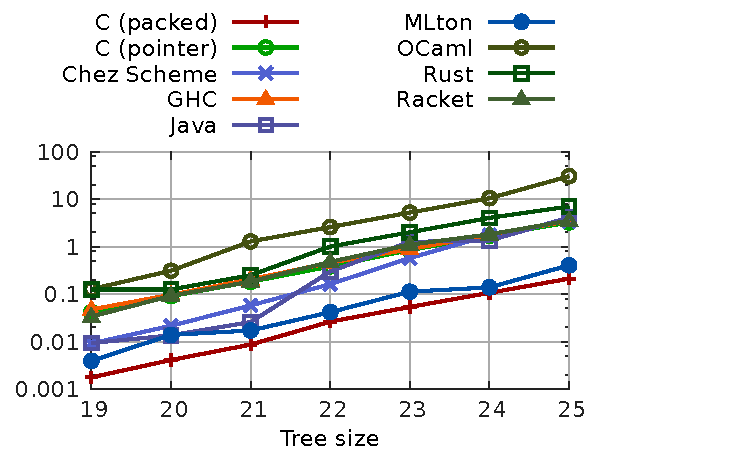
\includegraphics[width=4.4in]{./figs/shootout_add1.pdf}
%  \vspace{-4mm}
%   \end{minipage}

\begin{minipage}{1.02\textwidth}
\hspace{-5mm}      
  \begin{minipage}{.48\textwidth}
    \centering
    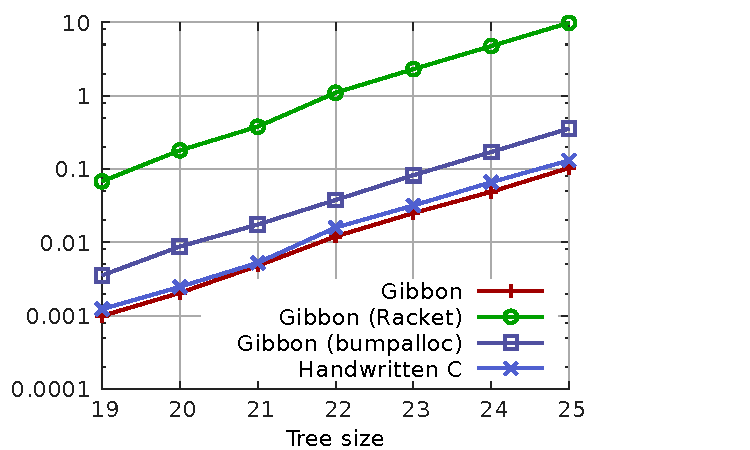
\includegraphics[width=3.75in]{./figs/shootout_buildtree.pdf}    
%    \label{fig:}
  \end{minipage}
  \hspace{3mm}
  \begin{minipage}{.48\textwidth}
    \centering
        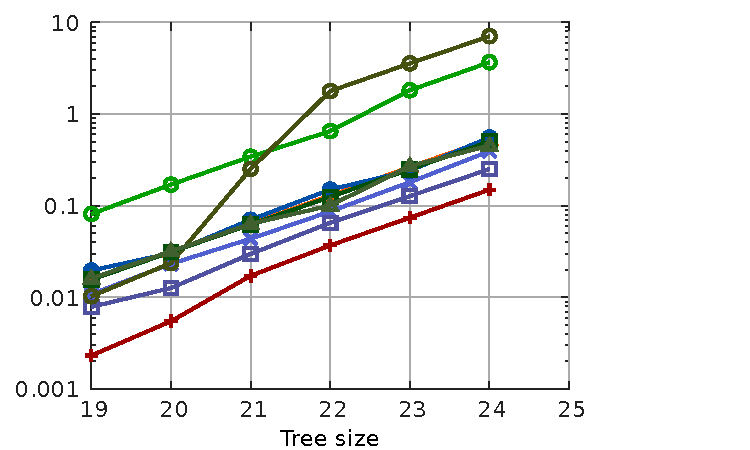
\includegraphics[width=3.75in]{./figs/shootout_sumtree.pdf}
%    \label{fig:}
  \end{minipage}

\end{minipage}
%  \vspace{-3mm}
  \caption{Performance when building (left), mapping add1 (top), and summing
    (right) a tree respectively.  Traditional compiler approaches vs. the packed
    approach.  All handwritten implementations.  X axis is tree {\em depth},
    implying $2^N$ leaves.  Y axis shows time in seconds.}
  \label{fig:shootout1}
\end{figure}

Figure~\ref{fig:shootout1} shows the results for these three microbenchmarks on
purely {\em handwritten} implementations, while varying tree size.
The results show a clear advantage for
packed representations (note the log scale), in some cases with 100x speedup
over pointer-based representations in garbage-collected languages.  All
competing implementations use their default memory management settings,
including GC parameters as well as the ``C (pointer)'' using the system malloc.

\begin{figure}[t]
  %  \vspace{-2mm}
  %\begin{figure}[]
  \hspace{5mm}
  \centering
  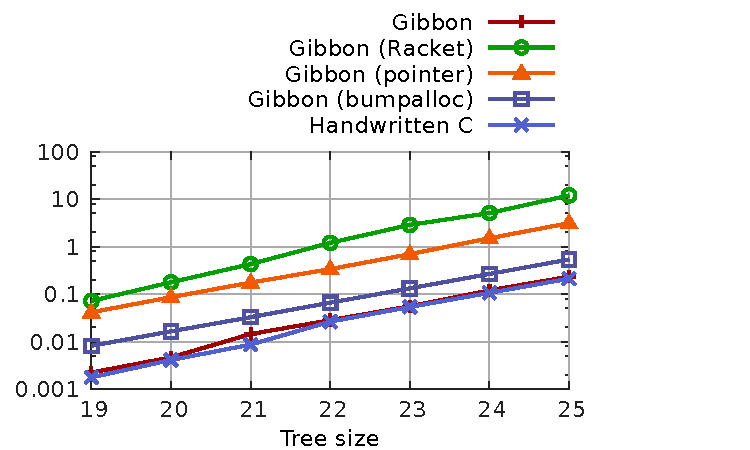
\includegraphics[width=4.3in]{./figs/shootout_treebench_five.pdf}
%  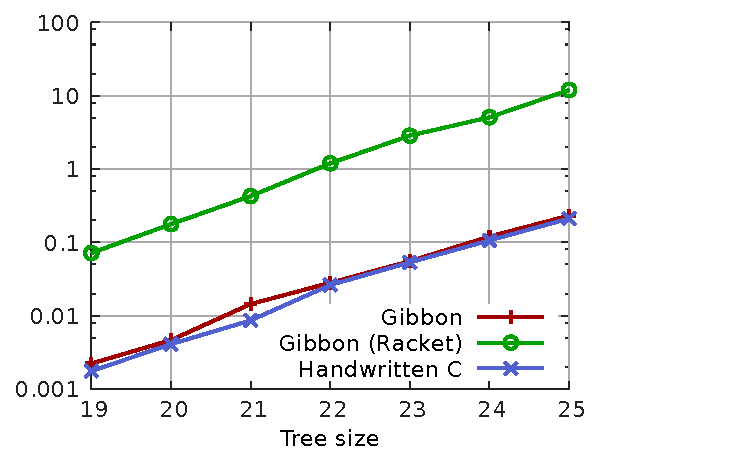
\includegraphics[width=4.8in]{./figs/shootout_treebench.pdf}
%   \label{fig:shootout2B}
%   \vspace{-4mm}
%\end{figure}

  \hspace{-6mm}  
\begin{minipage}{1.00\textwidth}
  \begin{minipage}{.49\textwidth}
    \centering
    %   \includegraphics[width=\textwidth]{./figs/.pdf}
       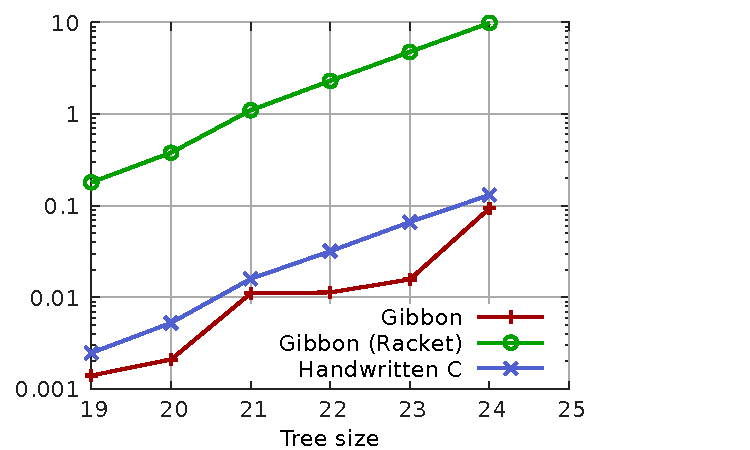
\includegraphics[width=3.8in]{./figs/shootout_gibbon_buildtree.pdf}
%        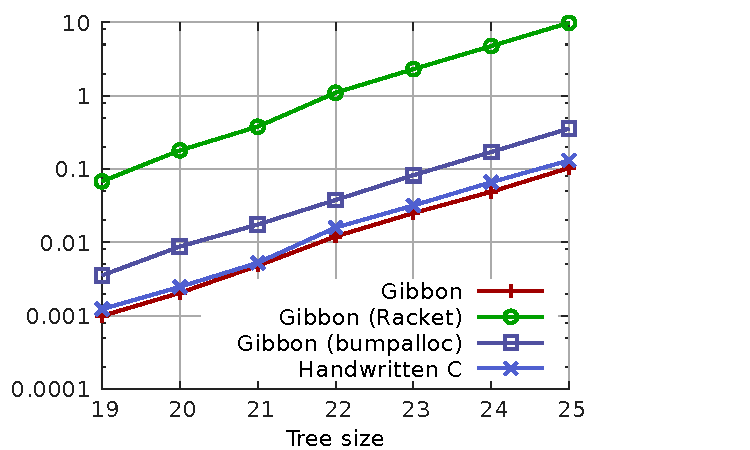
\includegraphics[width=3.8in]{./figs/shootout_gibbon_buildtree2.pdf}
%    \label{fig:}
  \end{minipage}
  \hspace{0.03\textwidth}
  \begin{minipage}{.49\textwidth}
    \centering
    %   \includegraphics[width=\textwidth]{./figs/.pdf}
%    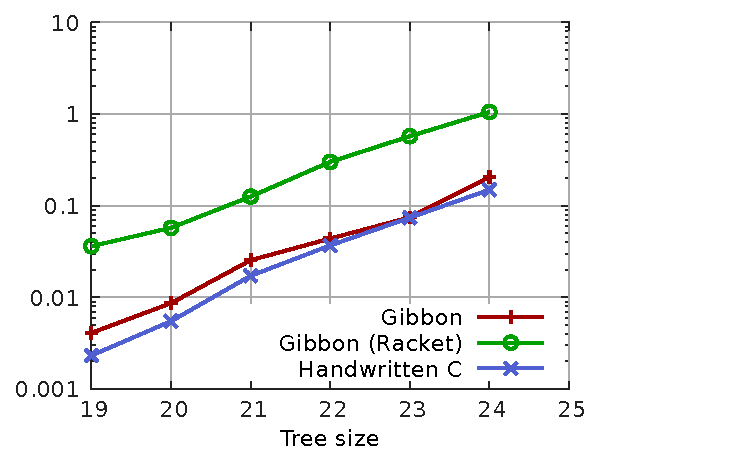
\includegraphics[width=3.8in]{./figs/shootout_gibbon_sumtree.pdf}
    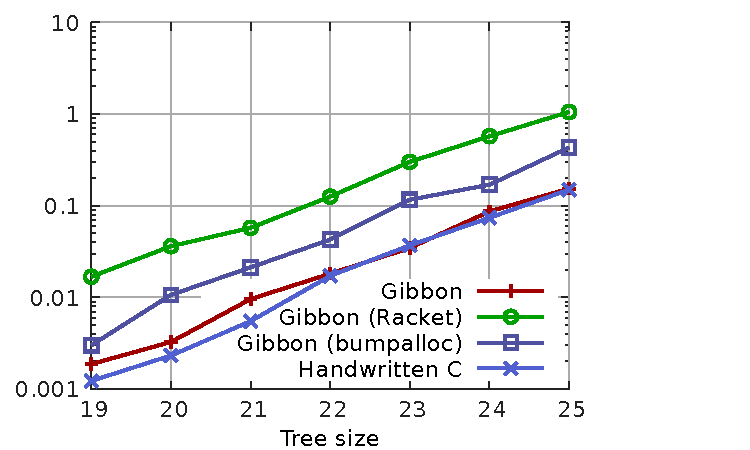
\includegraphics[width=3.8in]{./figs/shootout_gibbon_sumtree2.pdf}
%    \label{fig:}
  \end{minipage}
\end{minipage}
%   \vspace{-4mm}
   \caption{Cursor-inserting compiler's performance compared to handwritten
     cursorized C implementation.  Tree building (left), tree summing (right),
     and mapping add1 over the tree (top). The Gibbon prototype is currently
     embedded in Racket, so we show its Racket backend as well, as different
     modes of its C backend (packed, pointer, bumpalloc).}
   \label{fig:shootout2}
%   \vspace{-4mm}
\end{figure}


%% Our first ``shootout'' demonstrates the performance gains afforded by the
%% packed representation.
We next implement the tree building and summing benchmarks in \treelang{}, and
use our prototype cursor-inserting compiler to generate code over packed
representations.
% 
Figure~\ref{fig:shootout2} shows the results of comparing this
generated code to the handwritten C version of the packed representation
(because \treelang{} is embedded in Racket, we also show the results of direct
execution in Racket).
%
{We see that our compiler generated code that is competitive with, and
  occasionally exceeds, hand-written C code for the purpose of {\em packed} tree
  traversals.}
% \rn{That's not the point... finish this}

{Figure~\ref{fig:shootout2} shows build, mapping over, and summing a tree, separately.
%% In \cref{fig:shootout2B}, we show the add1-to-leaves function, which both
%% consumes and produces a tree.
  Here we introduce a couple of additional variants, which we will carry into
  the next section.  First, the {\bf pointer} version of Gibbon, as explained in
  \cref{sec:packed-pointer}, uses the same code generator but does not pack
  trees.  This version is faster than the Racket backend, but much slower than
  packed.  However, there is one more mode of the Gibbon code generator, {\bf
    bumpalloc}, also described in \cref{sec:packed-pointer}, which shrinks the
  gap further.  bumpalloc uses the same representations as pointer, but
  approximates optimal memory management with cheap arena allocation.  Still, it
  remains the case that on add1, packed yields a geomean speedup 1.75$\times$
  over bumpalloc, and 18$\times$ faster than the malloc-based pointer.}



\paragraph*{The influence of leaf size}
% \note{REMAINDER OF THE BUMPALLOC/PACKED RESULTS HERE}

In our simple tree example, we have thus far used a single @Int@ as the payload
of the leaf.  This implies a certain, fixed ratio of payload bytes to the memory
used for storing the structure of the tree---i.e., just tags in the packed
representation, or tags and pointers in a traditional representation.
%
We would expect that increasingly ``heavy'' nodes with many scalar fields, would
directly reduce the advantage of the packed representation.
% (Indeed, we see this again in \cref{sec:eval-kdtree}.)
To verify this hypothesis, we ran a simple parameter study where we generated
alternate versions of the @Tree@ data type and add1 traversal over it, varying
the number of @Leaf@ fields.
\cref{fig:vary-leaves} shows the results.
%
As expected, the best performance of the packed approach is with {\em zero}
leaves, and the performance of the ``bumpalloc'' version catches up as the
scalar payload of leaves increases.

\begin{figure}[t]
%  \vspace{-2mm}
  \hspace{-4mm}
  \begin{minipage}{1.04\textwidth}
    \begin{minipage}{.49\textwidth}
      \centering
      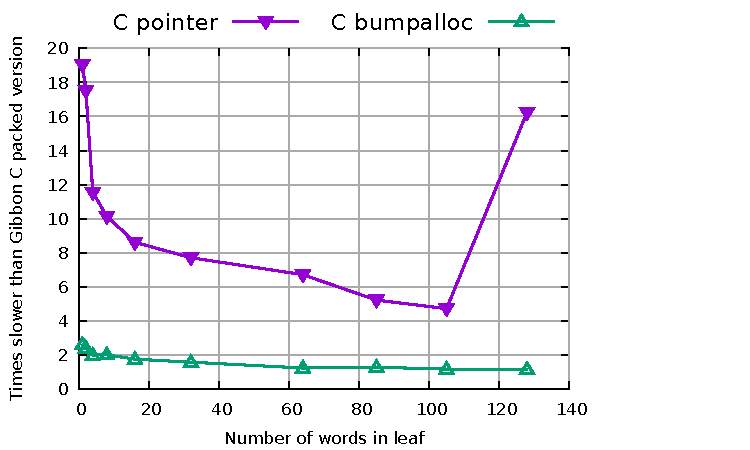
\includegraphics[width=3.8in]{./figs/slowdown_leaves_build.pdf}
    \end{minipage}
    \begin{minipage}{.49\textwidth}
      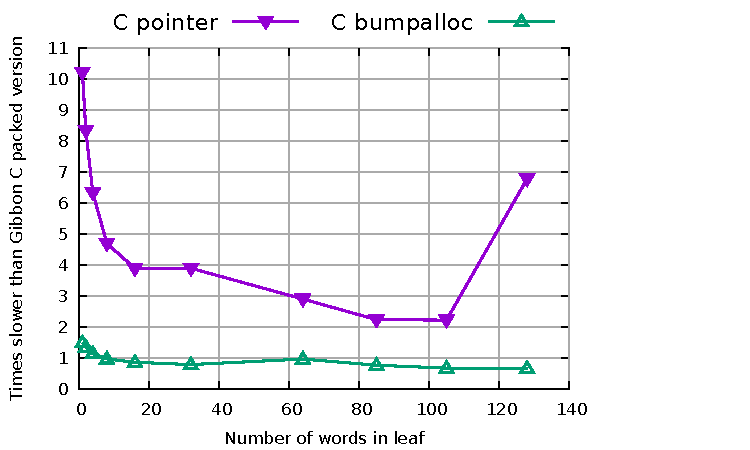
\includegraphics[width=3.8in]{./figs/slowdown_leaves_add1.pdf}
    \end{minipage}
  \end{minipage}
  \vspace{-4mm}
  \caption{The factor {\em slowdown} of competing approaches compared to a
    baseline of Gibbon's packed mode.  The malloc-based implementation performs
    especially badly when given large structs of over 800 bytes each.}
  \label{fig:vary-leaves}
%  \vspace{-4mm}
\end{figure}


%\note{A ``language shootout'' of add1-tree benchmarks.}

% \subsection{Old text - take or leave}
% 
% While our \treelang{} compiler is still a prototype, we already have
% promising results on simple programs. We compared three programs on
% binary trees of 64-bit integers: one program which constructed a tree,
% one program which adds 1 to each leaf, constructing a new tree, and
% one program which sums the elements of a tree.
% 
% In order to validate our packed data structure approach separately
% from our compiler implementation, we began with hand-written versions
% of each program across a range of language implementations, and
% implemented the programs with both packed and typical pointer-based
% techniques. The results of these experiments, plotting runtime versus
% the size of the tree in logaritmic scale, are seen in
% Figure~\ref{fig:shootout1}.
% 
% These results demonstrate two things. First, as simple data
% structure and memory management benchmarks, allocation performance is
% critical and modern safe languages perform well compared to C with
% \texttt{malloc()}/\texttt{free()}.
% %
% %% Second, packed implementations are
% %% a major speedup \emph{across multiple languages}, with consistent wins
% %% ranging from 2x to 10x.
% %
% Second, our low-level packed C implentation is
% consistently fastest, suggesting that a mature compiler following our
% strategy should perform well. 
% %
% We then tested our cursor-inserting \treelang{} compiler on these same
% benchmarks, comparing it to the handwritten packed C implementation
% (the fastest handwritten version from the previous figure). These
% results are plotted in Figure~\ref{fig:shootout2}. The results show
% that our compiler approaches or exceeds the performance of
% handwritten C code, despite it being a simplified prototype. Since this
% C program is already many times faster than a conventional
% implementation of these programs in a safe, functional, language, this
% strongly points to the potential of our approach.



\subsection{Compiler passes on realistic inputs} \label{sec:astbench}
% --------------------------------------------

While our microbenchmarks demonstrate the potential of the packed
representation, and also demonstrate \treelang{}'s ability to automatically
generate code that operates on the packed representation from idiomatic
implementations, they don't demonstrate a large savings of programmer effort,
because directly implementing functions on simple data in a packed
representation is tractable.

More challenging, however, is to operate on trees that have more complex
structure, such as the abstract syntax trees (ASTs) that arise in full blown
programming languages: (i) the trees themselves do not have homogeneous structure, so the
location of a particular tree node in a packed buffer is intimately related to
the types of the other nodes in the tree; and (ii) the operations on the tree
nodes are not homogeneous, so the structure of computations (including how to
extract particular fields from a serialized representation of a tree node)
varies based on the type of the tree node. In this setting, writing a tree
traversal that operates directly over a packed representation is complex and
error prone. On the other hand, writing such a traversal in an idiomatic style
using pattern matching is fairly straightforward. This, then, is an ideal use
case for \treelang{}'s approach.

\paragraph*{Benchmarks}
In this portion of the evaluation, we look at
% two compiler passes, each of which takes a
the performance of two classes of tree walk
% (a fold and a map)
on full Racket Core syntax, an AST definition which is excerpted in \cref{fig:racket-core}.
%
These benchmarks consume a Racket abstract syntax tree as input and produce
either (1) a count of nodes, or (2) a new abstract syntax tree.
% The two passes are copy propagation and substitution.
%% In both cases, the structure of the output AST might differ from that of the
%% input AST.
%
While we only evaluate two simple treewalks,
%% \footnote{An artifact of  \treelang{}'s prototype compiler's limitations, not \treelang{}'s
%%   expressiveness.}
we note that these traversals contain the two major operation
types that might be performed on trees: {\tt map}s, where the output tree is
structurally similar to the input tree but with a function applied to each node,
and {\tt fold}s, which in this context is transforming an entire subtree into
some differently-structured result.
%
Seen at this high level, all compiler passes on ASTs
are roughly similar, differing mostly in the work done near the leaves of
trees.
%
For example, substitution, copy-propagation, and constant folding all traverse a
tree and ``act locally''.  In general, many transformations only transform a
small fraction of the input and spend most of their time simply walking over syntax.
%
%% Hence, we expect the results of these two traversals to be representative for
%% map-like passes and simple analysis passes (folds).


We write both benchmarks in \treelang{}. We then generate versions of each
benchmark, as before, one using \treelang{}'s {\em pointer-based} backend (which
generates passes over pointer-based ASTs in C), and one using \treelang{}'s
{\em packed} backend. By letting the
implementations differ only in the backends used to generate them, we isolate
the performance differences to those that arise from the difference in
representation. Because \treelang{} allows tree traversals to be written
using standard data type match operations, this evaluation also
serves to confirm our ability to generate packed implementations from
idiomatic code.

We generated a dataset of inputs by collecting all of the (macro-expanded) source
code from the main Racket distribution, which contains 4,456 files consuming
1GB of code which drops to 485MB when stripped of whitespace and comments, and 
102MB once packed in our dense representation.
% (disregarding symbol tables).
%
We benchmark on this entire dataset, but report only on a subset, sampling from
a spectrum of sizes.
%
The largest single file was 1.4MB. 
To simulate larger programs (as would be found in whole-program compilation), we
combined the largest $K$ files into one, varying $K$ from 1 to 4,456.
%
This is representative of a whole program compiler, which would indeed need to
load these modules as one tree.
%
%% ranging in size from {XXX nodes to YYY nodes, with ZZZ different inputs},
%% overall. Note that these inputs represent real-world programs of varying sizes,
%% ranging from XXX bytes to YYY bytes.
%
%% This range of programs and sizes allows us
%% to understand how input-dependent the behavior of our cursor passing
%% transformations and our packed representations are, as well as confirm that our
%% approach works across a wide range of real inputs.

\paragraph*{Results}

First, our benchmark methodology is to traverse each input tree $N$ times,
doubling $N$ until the run takes at least two seconds.  This gives us a uniform
way of measuring both traversals over very small trees and very large ones.


\cref{fig:slowdown} shows the performance of Gibbon's packed mode vs gibbon's
pointer (malloc) and bumpalloc modes, expressed as slowdowns of the pointer-based approaches over packed.  We measured the last level cache
reference and cache misses and found dramatic improvements in these for the
packed approach (and modest differences in the number of instructions executed).
%
Nevertheless the performance of pointer-based approaches is good at small
sizes: (1) trees are small and fit in cache, (2) the single threaded workload
can acquire all of the last level cache, not contending with other threads on
the 16-core machine.  The end result is that the system is able to mask the bad
behavior of these implementations at these sizes.
%
When the input/output tree sizes exceed the cache size, however, we see a phase
shift.  Once we need to stream trees from memory, the smaller memory footprints
and linear access patterns of Gibbon's packed approach yield speedups of
2.5-3$\times$ for fold and 2$\times$ for map.

%% \Red{Figures~\ref{fig:copyprop} and~\ref{fig:subst} present the results
%% for copy propagation and substitution, respectively. The x-axis of each figure
%% shows the different possible inputs, ordered by the speedup of the packed
%% version over the pointer version (higher is better). The dashed horizontal
%% line on each figure represents the geomean speedup across all inputs.

%% We see \note{something -- describe these figures once we see them!}

% \note{Are we also going to show the same charts ordered by size, instead?}



%% \subsection{Typechecking benchmark}
%% % --------------------------------------------

%% \note{type check the simply-typed $\lambda$ calculus in \treelang{}}

\begin{figure}[t]
%  \vspace{-2mm}
  \hspace{-5mm}
  \begin{minipage}{1.04\textwidth}
    \begin{minipage}{.49\textwidth}
      \centering
      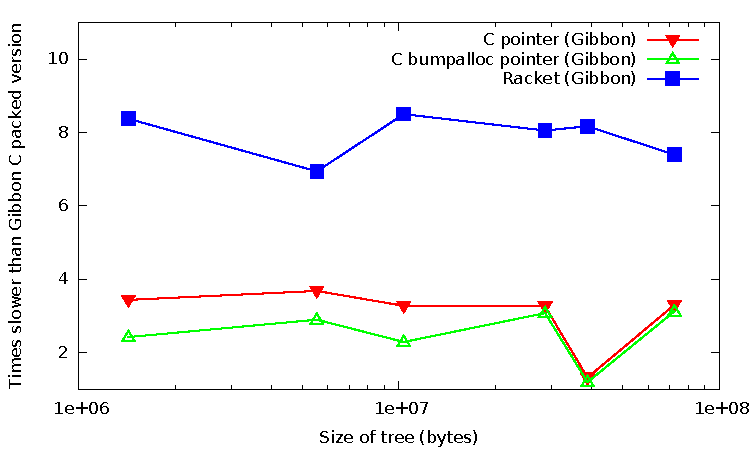
\includegraphics[width=3.8in]{./figs/slowdown_countnodes.pdf}
    \end{minipage}
    \begin{minipage}{.49\textwidth}
      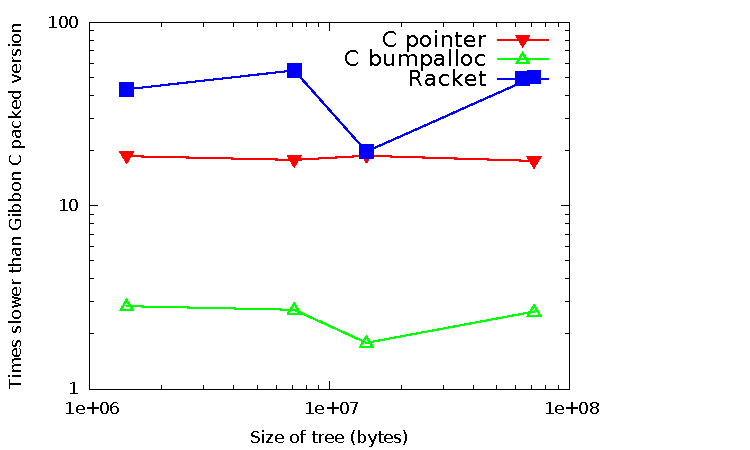
\includegraphics[width=3.8in]{./figs/slowdown_treewalk.pdf}
    \end{minipage}
  \end{minipage}
%  \vspace{-4mm}
  \caption{The factor {\em slowdown} of competing approaches compared to a
    baseline of Gibbon's packed mode.  The X axis is the size in bytes of the
    (packed) input tree.  Left is the fold benchmark which counts the AST nodes
    in the tree.  On the right is a map over the tree.}
  \label{fig:slowdown}
%  \vspace{-4mm}
\end{figure}
      
%% This works well in footnotesize
%% {\begin{figure}
%%   \begin{code}   
%%  data Expr = VARREF Sym                     data Toplvl = DefineValues   ListSym Expr 
%%            | Lambda Formals ListExpr	                | DefineSyntaxes ListSym Expr  
%%            | CaseLambda LAMBDACASE                      | BeginTop ListToplvl         
%%            | If Expr Expr Expr                          | Expression Expr             
%%            | Begin ListExpr
%%            | Begin0 Expr ListExpr           
%%            | LetValues    LVBIND ListExpr   data Formals = F1 ListSym    
%%            | LetrecValues LVBIND ListExpr                | F2 ListSym Sym
%%            | SetBang Sym Expr                            | F3 Sym        
%%            | Quote Datum
%%            | QuoteSyntax Datum
%%            | QuoteSyntaxLocal Datum
%%            | WithContinuationMark Expr Expr Expr
%%            | App Expr ListExpr 
%%            | Top Sym
%%            | VariableReference    Sym 
%%            | VariableReferenceTop Sym 
%%            | VariableReferenceNull
%%     ....
%%   \end{code}


{\begin{figure}[t]
  \begin{code}   
 data Toplvl = DefineValues   ListSym Expr 
             | DefineSyntaxes ListSym Expr 
             | BeginTop ListToplvl         
             | Expression Expr             
             
 data Expr = VARREF Sym                     
           | Lambda Formals ListExpr	     
           | CaseLambda LAMBDACASE          
           | If Expr Expr Expr              
           | Begin ListExpr
           | Begin0 Expr ListExpr           
           | LetValues    LVBIND ListExpr   
           | LetrecValues LVBIND ListExpr   
           | SetBang Sym Expr               
           | Quote Datum
           | QuoteSyntax Datum
           | QuoteSyntaxLocal Datum
           | WithContinuationMark Expr Expr Expr
           | App Expr ListExpr 
           | Top Sym
           | VariableReference    Sym 
           | VariableReferenceTop Sym 
           | VariableReferenceNull
    ....
  \end{code}



%% (data Toplvl
%%       [DefineValues   ListSym Expr]
%%       [DefineSyntaxes ListSym Expr]
%%       [BeginTop ListToplvl]
%%       [Expression Expr])

%% (data Expr
%%       (VARREF Sym)              
%%       (Lambda Formals ListExpr)	
%%       (CaseLambda LAMBDACASE)
%%       (If Expr Expr Expr)
%%       (Begin ListExpr)
%%       (Begin0 Expr ListExpr)
%%       (LetValues    LVBIND ListExpr)
%%       (LetrecValues LVBIND ListExpr)
%%       (SetBang Sym Expr)
%%       (Quote Datum)
%%       (QuoteSyntax Datum)
%%       (QuoteSyntaxLocal Datum)  ;; (quote-syntax datum #:local)
%%       (WithContinuationMark Expr Expr Expr)
%%       (App Expr ListExpr) 
%%       (Top Sym)
%%       (VariableReference    Sym) 
%%       (VariableReferenceTop Sym) 
%%       (VariableReferenceNull))
      
%% (data LVBIND
%%       (CONSLVBIND ListSym Expr LVBIND)
%%       (NULLLVBIND ))

%% (data LAMBDACASE
%%       (CONSLAMBDACASE Formals ListExpr LAMBDACASE)  ;; (formals expr ...+) 
%%       (NULLLAMBDACASE ))

%% ;; RRN: How far do we need to go here?
%% (data Datum
%%       (INTLIT Int)
%%       ; (SYMLIT Sym)
%%       ; (CONS Datum Datum)
%%       ; (NULL)
%%       )

%% (data Formals
%%       [F1 ListSym]        ;; Tag 0
%%       [F2 ListSym Sym]    ;; Tag 1
%%       [F3 Sym])                ;; Tag 2

%% (data ListToplvl
%%       (CONSTOPLVL Toplvl ListToplvl)
%%       (NULLTOPLVL))

%% (data ListExpr
%%       (CONSEXPR Expr ListExpr)
%%       (NULLEXPR))

%% (data ListSym
%%       (CONSSYM Sym ListSym)
%%       (NULLSYM))

  \caption{Excerpt of Racket Core AST definition in Gibbon., which 
   follows \url{https://docs.racket-lang.org/reference/syntax-model.html}.
   There are nine data types total.}
  \label{fig:racket-core}
\end{figure}}



\section{Extensions}
%============================================================================
\label{sec:extensions}

This section evaluates two extensions to \treelang{} that enable more complicated traversals and expose more opportunities for performance.

Our benchmarks up until now focus on ``full'' treewalks: traversals that visit
every node of the input tree, in order. While this assumption is accurate for
most compiler passes, there are some scenarios and applications where this may
not be true:
\begin{itemize}
  \item If a traversal exploits {\em truncation}. Some tree traversals, such as those of space partitioning trees~\cite{gray2000n} gain asymptotic improvements by {\em truncating} traversals of subtrees. Based on some condition (for example, that a given subspace in a space partitioning tree is unimportant), traversal of a node's entire subtree is skipped, and the traversal continues on to the sibling of the current node. This optimization means that not all of the tree is visited by the traversal.
  \item If a traversal is {\em parallelized}. To run a traversal in parallel, multiple threads collaborate to walk over a tree. In many traversals, this parallelism is natural: walks over different subtrees are independent of each other. In {\em this} scenario, a single thread may not walk over the entire tree and, indeed, may not even start its tree walk at the beginning of the buffer holding the tree.
\end{itemize}

For both of these cases, our current \treelang{} compiler is insufficient,
because it does not support non-full treewalks. It assumes that the
cursor moving through the buffer runs by each node in the tree during the tree
walk, and the transformations that ensure that cursors get routed correctly
assume the same. The key distinction here is that in both the truncation case
and the parallelism case, we need some way to move a cursor to (or generate a
cursor at) some later point in a packed tree buffer {\em without} walking over
the intermediate tree nodes.

This section describes an extension to \treelang{}'s packed representation---{\em layout information}---that enables these more sophisticated traversals, as well as a evaluation of two benchmarks that use this extended representation.

\subsection{Adding Layout Information for Indirection}

As described in Section~\ref{sec:copy-insert}, our current approach for
handling traversals where we need a cursor position (e.g., the position of a
right child) without an accompanying traversal that generates it---in other
words, if we need to skip over a portion of the tree---is to insert a dummy traversal that traverses the portion of the tree we are skipping. This
dummy traversal generates the required cursor position to continue with the
``real'' traversal. However, this approach can be inefficient if the amount of work
done by the dummy traversal is large: in the original pointer-based code, a
traversal has direct access to all children, and can hence immediately skip
over any subtrees that are unnecessary, whereas code using the packed
representation must traverse the entire tree at all times. In some situations,
these dummy traversals can turn $O(\log n)$ operations into $O(n)$ ones,
an unacceptable increase in complexity (consider, for example, the {\tt right} example from Section~\ref{sec:limitations}).


Our solution to this problem is the introduction of {\em indirections} in the
packed representation. These are, effectively, values stored in the packed
tree that can be used to generate necessary cursor positions without
performing traversals. This layout information amounts, essentially, to adding
pointers to our packed representation (albeit ones that only have to be used
in lieu of dummy traversals). However, they still preserve some of the space
benefits of the packed representation for three reasons. First, indirections
are not necessary for the first child, as it is placed immediately after its
parent. Second, indirections are
only necessary during some portions of traversal; if a particular type of node
does not have computations that require skipping subtrees, there is no need to
add indirections to that type of node. Third, even if indirections {\em are}
required everywhere, they are only required to be offsets within the buffer,
not full (64-bit) pointers, which can enable space savings.

The particular type of indirection needed depends on the mechanism of the
traversal. Here,
we discuss two common patterns.

\begin{description}
  \item[Pointer-style indirection] The most common type of indirection is a
  ``pointer style'' indirection, where the indirection serves to provide easy
  access to children beyond the first child: a node contains a field that
  contains the size of the left subtree. Adding that value to the current
  cursor allows the cursor to be moved past the left subtree and on to the
  right subtree. These types of indirections are useful to quickly access,
  say, the right child of a node without traversing the left child's subtree.
  The {\tt right} code example from Section~\ref{sec:limitations} can benefit
  from a pointer-style indirection.
  \item[Rope-style indirection] This is a more subtle style of indirection. In
  some types of tree traversals (such as those that arise in n-body
  codes~\cite{gray2000n}), an interior node is visited and, based on some {\em
  data-dependent} condition, either both children of the interior node are
  visited or {\em neither} is visited, effectively truncating the traversal of
  both the left and the right subtrees. This truncation effectively serves as
  a data-dependent base case for a recursive traversal. We call these {\em
  rope-style} indirections because these types of indirection pointers are
  frequently called ``ropes'' when used in GPU implementations of tree
  traversals~\cite{goldfarb13sc,popov07,hapala11}. An indirection pointer
  captures the size of both the left and right subtrees (generalizing, all
  child subtrees) of a node, allowing the cursor to be bumped to the necessary
  location upon truncation.
  
  Interestingly, \treelang{}'s packed representation makes finding the next
  node easy---a simple calculation of the size of subtrees. In pointer-based
  representations, finding the next node of the tree requires more work: it
  could be the right sibling of the current node, it could be the node's
  parent's right sibling, etc.
\end{description}

Note that in both cases, the indirection pointer's main job is to capture the
size of a subtree or subtrees rooted at a particular node. In general, if a
given interior node knows the sizes of all of its child subtrees, it can use
these indirection pointers to provide {\em random access} to a tree, even if
that tree is in a packed representation. Hence, we call this indirection
information {\em layout information}.

Not every traversal requires full random access to the tree, and hence not
every piece of layout information is necessary to synthesize traversals over
packed trees.
Automatically inferring what layout information is necessary,
inserting them into packed representations, and synthesizing cursor updates based on that layout information is a topic for future work.


\subsection{Evaluation}%\label{sec:eval-parallelism}
\label{sec:eval-extensions}

Because \treelang{} does not currently support a packed representation
extended with layout information, our evaluation uses hand-written packed
implementations (in C) that include that layout information, mimicking what
would be produced by a backend that understands indirections. We evaluate two
benchmarks: a {\em parallelization} microbenchmark
(Section~\ref{sec:eval-parallelism}) that uses pointer-style indirections to
distribute the traversal of a tree, and an implementation of {\em two-point
correlation} (Section~\ref{sec:eval-kdtree}) that uses rope-style
indirections.

\subsubsection{Parallelism opportunity study} \label{sec:eval-parallelism}
\label{sec:eval-parallel}
% ---------------------------------------------------------------------

We evaluate a {\em parallel} version of our {\tt add1} benchmark from
Section~\ref{sec:microbench}. In the pointer-based version of this code,
adding parallelism using Cilk~\cite{cilk} is straightforward: because the {\tt
add1} operation treats the left and right subtrees independently, we can
simply add Cilk {\tt spawn} commands to recursive calls to introduce
parallelism, cutting off parallelism as necessary to avoid runtime overhead.

For the packed representation, however, we cannot simply adopt this approach:
being able to {\tt spawn} a task that processes the right subtree of a node
requires being able to reach that right subtree {\em without traversing the
left subtree}. We thus manually introduce {\em pointer-style} indirections
that allow programs written over the packed representation to directly access
the right subtree, facilitating parallel execution. In any scenario where
there is a Cilk {\tt spawn}, we use the indirection pointer to launch the
right-subtree task, allowing that work to be stolen. Once we cease using {\tt
spawn}s, producing coarse-grained leaf tasks, we revert to the full tree-walks
supported by \treelang{}.

\begin{figure}[t]
  \vspace{-5mm}
% \begin{minipage}{1.04\textwidth}
    \centering
  \begin{minipage}{.75\textwidth}
    \centering
%    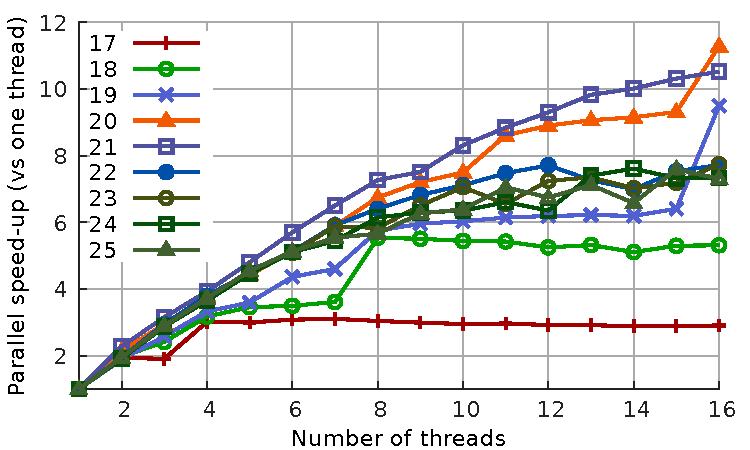
\includegraphics[width=\textwidth]{./figs/speedup_cilk.pdf}
    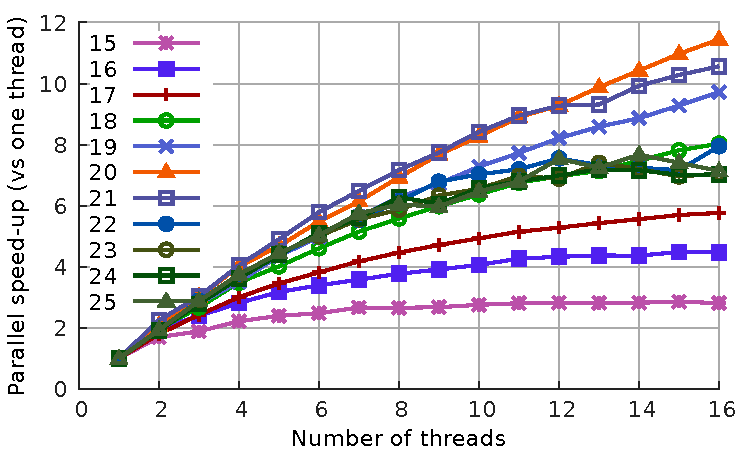
\includegraphics[width=\textwidth]{./figs/speedup_handwritten-c-packed-cilk_cutter_pardepth8.pdf}    
%    \label{fig:}
  \end{minipage}
  %  \hspace{0.1\textwidth}
  $ $ 
  \begin{minipage}{.75\textwidth} 
    \centering
    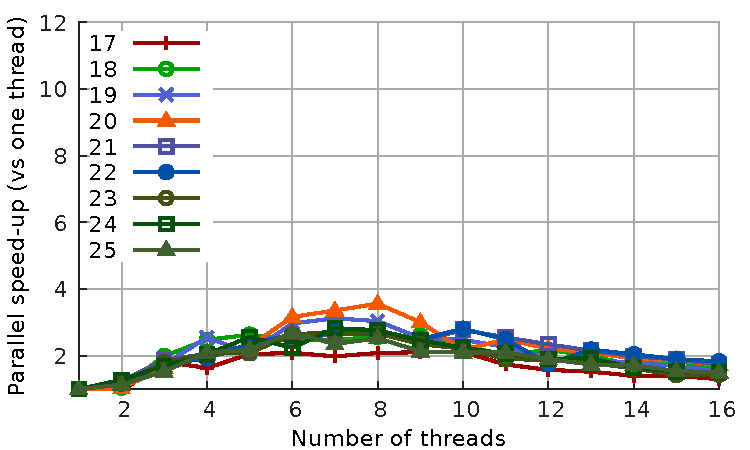
\includegraphics[width=\textwidth]{./figs/speedup_ghc.pdf}
    % \includegraphics[width=60mm]{example-image-b}
%    \label{fig:}
  \end{minipage}
%\end{minipage}
  \caption{Parallel speedup: mapping a function over a packed tree.
    Each line is labeled with the tree depth that it represents, including
    trees of $2^{15}$ to $2^{25}$ leaves.
     This
     compares a Cilk (C) implementation using the packed trees with layout information
     that allow random access to subtrees (left).  For comparison, we also show
     the parallel speedup from a mature parallel functional compiler (GHC,
     right).  All lines are normalized to their own 1-core speeds.  In absolute
     terms, GHC starts off 34$\times$ slower than our approach at one core, and
     grows to 223$\times$ slower at 16 cores.}
   \label{fig:par-shootout}
%      \vspace{-4mm}
\end{figure}
% C/1 0.0036089296875
% HS/1 0.1226078125,
% (/ 0.1226078125 0.0036089296875 ) 34 times

% C/16    0.000319918212890625
% HS/16   0.07138175
% (/ 0.07138175 0.000319918212890625) 223 times


Figure~\ref{fig:par-shootout} shows the result of our parallel packed
implementation (left), compared to the performance of a mature parallel
functional compiler, GHC, running the same benchmark (right). While for small
trees we see that our parallel implementation does not yield much scaling, for
large trees we can achieve a speedup of about 11$\times$ on 16 cores (relative
to one-core execution). In contrast, the GHC implementation cannot scale
beyond eight cores.
%
At these allocation rates, GHC spends much of its time in garbage
collection, and the runtime system presents a bottleneck.
% \footnote{Unfortunately, GHC, as of 8.0, has a non-scalable  stop-the-world collector.}
%
When comparing the packed implementation directly to 
GHC, the packed version is 34$\times$ faster on a single core
and 223$\times$ faster on 16 cores!

While automatically exploiting parallelism in \treelang{} is future work, these results
demonstrate the potential for large performance gains.

% \note{Report preliminary parallel microbenchmark results, showing the potential
%   for future work here.}
% 
% \note{ A final goal of this project is to explore the role
% {these alternate CNF and DPNF} representations can play in parallelizing programs.
% \Cref{fig:shootout2} shows how a hand-parallelized version the packed approach
% scales much better than a traditional functional compiler.  We believe this
% approach has great potential for improving both single core and multicore performance.
% \Cref{fig:par-shootout}.............}


\subsubsection{Point correlation} \label{sec:eval-kdtree}
% --------------------------------------------
Point correlation  is a well-known algorithm used in data mining~\cite{gray2000n}:
given a set of points in a k-dimensional space, point correlation computes the number of points in that space  that lie within a
distance r from a given point p. 

% Rather than comparing each point in the space to the query point, one efficient way of searching such spaces is to store them in kd-trees~\cite{bentley75}. KD-trees are space partitioning trees where the root of the kd tree represents the entire space, and each node's children represents a partition of that node's space into two subspaces.

% A kd-tree is a binary space partitioning tree that in its simplest form  splits the space at each internal node into two sub-spaces
% around a split axes in one of the space dimensions, the left subtree stores the points to the left of the split access
% and the right subtree sotres the points to the right of the split access, the split axes alternates between the dimensions of
% the space at each level of the tree, when the number of the points in the subtree is one, a leaf node that stores
% that point is constructed.


In a naive implementation of point correlation, each point in the space needs
to be checked against the query point. 
A more efficient approach is to use kd-trees~\cite{bentley75} to store the points. KD-trees are space partitioning trees where the root of the kd tree represents the entire space, and each node's children represents a partition of that node's space into two subspaces.
KD-trees allow the search
process to skip some regions in the space. By storing at each internal node
the boundaries within which all descendent points lies, the search process can
skip a subtree is a given point is far enough from the boundaries. As a
result, querying a kd-tree to perform point-correlation is $O(log\; n)$ instead
of $O(n)$. Note that it is exactly the process of ``skipping'' subtrees that
gives kd-tree-based point correlation its efficiency, but also that prevents a
normal packed representation from sufficing to implement the algorithm: there
is no way to skip past a subtree without performing a dummy traversal,
obviating the asymptotic performance gains.

We implemented both a standard pointer-based version of 2-point correlation in
C, as well as a version that operates over a packed representation augmented
with indirection pointers. Each interior node stores a rope-style
indirection pointer that maintains the size of its child subtrees. If a
traversal is truncated at that node, the cursor is incremented by the value in
that indirection pointer, skipping the subtrees and resuming traversal on the
rest of the tree.

  
\begin{figure}[htp]
% \begin{minipage}{1.04\textwidth}
  % \begin{minipage}{.49\textwidth}
    \centering
    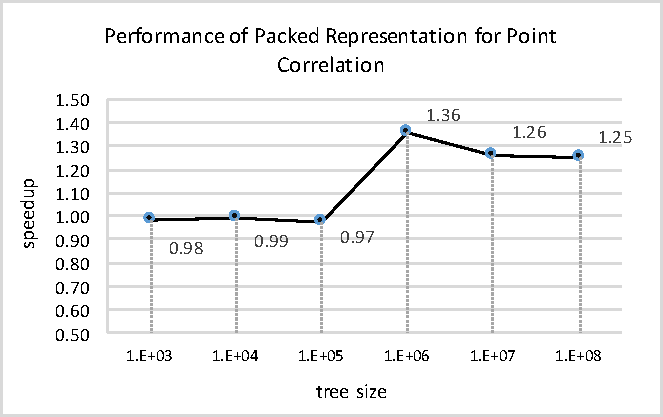
\includegraphics[width=0.7\textwidth]{./figs/pointCorr_perf.pdf}

  % \end{minipage}
  % $ $ 
  % \begin{minipage}{.49\textwidth}
    % \centering
    % 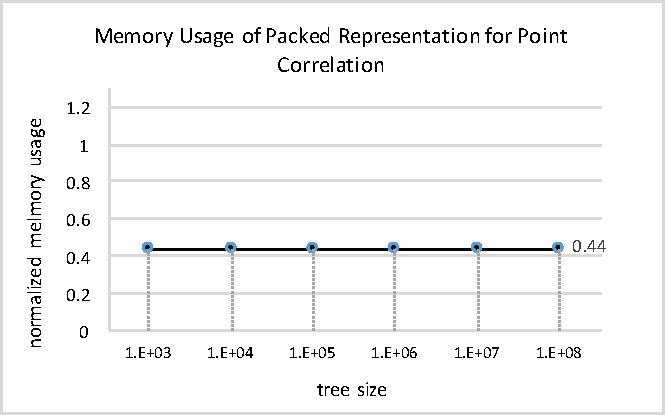
\includegraphics[width=\textwidth]{./figs/pointCorr_MemUsage.pdf}
    % \includegraphics[width=60mm]{example-image-b}
%    \label{fig:}

%   \end{minipage}
% \end{minipage}
   \caption{Speedup of packed implementation of point correlation over pointer-based implementation. X axis shows varying tree sizes (represented in number of nodes).}
         \label{fig:pointCorr}
\end{figure}

  
Figure \ref{fig:pointCorr} shows the speedup of the packed version with respect to the standard pointer-based implementation for different tree sizes. For each tree size, we ran 10 query points through the tree. For small trees, the queries were performed 10000 times to produce sufficient runtime for accurate measurements. Each experiment was performed 10 times, and the mean is reported. 

We note first that for every tree size, the packed representation uses 56\% less memory than the pointer-based trees. This reduction in memory usage has two sources: nodes do not need to store left-child pointers; and more efficient packing of data in the packed representation. For small trees, the runtime performance of the packed and pointer versions are comparable. For large trees, the packed version is 35\% faster than the pointer-based version.

We note that the relatively smaller performance improvement for this benchmark versus the AST benchmarks is unsurprising. First, taking an indirection means that any spatial locality gains from the packed representation are lost, resulting in similar behavior to the pointer-based version. Second, there is relatively more work to be done per node in this benchmark, so the time spent in traversal of the tree is relatively less, reducing the opportunity for improvement.
% 
%  We
% packed representation uses 56\% less memory to represents the tree than the pointer based representation, this reduction in memory usage has two sources;
% the elimination of the left child pointer and the elimination of the gaps between the structure data members that are added by default for memory alignment purposes.
% The runtime performance of the packed version is almost the same as the pointer based for small trees, however when the size of the tree is large enough the packed version 
% shows up to 35\% speed up.








% ================================================================================
\section{Future Work and Conclusions}
% ================================================================================
\label{sec:future}
\label{sec:conclusion}
\paragraph*{Future work}

While our initial results show that packed tree-based data
representation have significant promise for accelerating tree
transformations, much more work remains to be done. First,
our \treelang compiler remains an initial prototype---a more realistic
implementation supporting arrays, lists, and more base values would
allow the construction of more interesting programs, further
validating our hypotheses. We also plan to support optional automatic
inclusion of layout size information to enable applications such as
kd-trees directly in the \treelang language.

Further extensions to the simplest model of packed data provide the
promise of additional gains. One extension to the model is the
addition of \emph{indirection nodes}, allowing allocation of unknown
sizes by chaining together buffers, or supporting parallelism more
effectively with pointers at the top of a tree and dense packing
further down. Indirection nodes are a generalization of the indirections
described in Section~\ref{sec:extensions}: rather than pointing only to other
locations within the same buffer, an indirection node could point to a {\em
different} buffer.

Another extension is \emph{data type factoring}, storing
leaves in a separate, dense, aligned vector.  This enables (1)
vectorization of numeric operations, and (2) separating out pointers
that the GC must traverse.  This may prove essential for an open-world
implementation in a managed language such as Java, Haskell, or Racket,
where the low-level control provided by C is not possible, and
interoperation with arbitrary pointer-based values is desirable.

Finally, while our parallelism opportunity study shows that packed
data is an excellent approach to parallel computation, we have not yet
explored this further. Turning promise into reality will require
significant additional work.

\paragraph*{Conclusions}

This paper investigates the use of {\em packed} representations to represent
tree structures, which serialize a tree and eliminate the pointers connecting
the various nodes. While this representation saves space and, with
carefully-written code, can result in performance improvements (due to
prefetching and spatial locality), writing programs that operate directly on
the packed representation is challenging and error prone. To address this
problem, this paper introduces \treelang{}, a simple functional language and
compiler that allows programmers to write tree traversal algorithms in
standard, idiomatic ways (recursion over algebraic data types), and a compiler
that automatically generates the packed representation for an application and
transforms \treelang{} programs to operate directly on that representation.

We show through a series of microbenchmarks and case studies that our packed
representation is highly efficient compared to pointer-based representations,
both in terms of space usage and time, and that we can
%write even fairly complex compiler passes over
process complex data, such as the full Racket language's
ASTs in \treelang{}, and automatically translate
them to packed implementations. We also discuss extensions to \treelang{} that
introduces selective random access to tree nodes in packed representations,
opening up \treelang{} to more complex applications.

%% % ================================================================================
%% \appendix
%% \section{Appendix Title}
%% % ================================================================================

%% This is the text of the appendix, if you need one.

%% \acks

%% Acknowledgments, if needed.

% \bibliographystyle{abbrvnat}
\bibliographystyle{abbrv}

% If you can't commit to the submodule right this second, just copy
% this file to ./refs.bib :
\bibliography{bibs/refs}

% The bibliography should be embedded for final submission.
%% \begin{thebibliography}{}
%% \softraggedright
%% \bibitem[Smith et~al.(2009)Smith, Jones]{smith02}
%% P. Q. Smith, and X. Y. Jones. ...reference text...
%% \end{thebibliography}


\end{document}


